% To be used for generating only 1 chapter of the thesis

\title{Side-Channel Security in Networks: From the Internet to Interconnects}

\author{Rut Vora}
\previousdegree{B. Engineering in Computer Science, BITS-Pilani, 2020}


\degreetitle{Master of Science}

\institution{The University of British Columbia}
\campus{Vancouver}

\faculty{The Faculty of Graduate and Postdoctoral Studies}
\department{Computer Science}
\submissionmonth{March}
\submissionyear{2025}

\examiningcommittee{Aastha Mehta, Assistant Professor, Computer Science, \textsc{UBC}}{Supervisor}
% \examiningcommittee{Mathias L\'{e}cuyer, Assistant Professor, Computer Science, \textsc{UBC}}{Co-Supervisor}
% \examiningcommittee{Margo Seltzer, Professor, Computer Science, \textsc{UBC}}{Supervisory Committee Member}

%% hyperref package provides support for embedding meta-data in .PDF
%% files
\hypersetup{
  pdftitle={Side-Channel Security in Networks: From the Internet to Interconnects  (DRAFT: \today)},
  pdfauthor={Rut Vora},
  pdfkeywords={PCIe, CXL, Side Channels, Networks, Proxy}
}

\begin{document}

% \maketitle

\textspacing		% begin one-half or double spacing

% Body of Thesis (not all sections may apply)
\mainmatter

\acresetall	% reset all acronyms used so far

% Main Sections
% %% The following is a directive for TeXShop to indicate the main file
%%!TEX root = thesis.tex

\chapter{Introduction}
\label{ch:Introduction}

Today, we live in a connected world where various network links are used to transmit and receive a lot of data. 
This data can be a webpage or video being streamed by a user on the internet. 
It can also be an image or a machine learning model being sent from the CPU to the GPU for processing. 
Given the extensive scale at which data is transmitted, ensuring its security and privacy during transit is of paramount importance.

To protect data that is in transit, we have come to rely on encryption. 
Most encryption mechanisms today rely on mathematical functions that transform the plaintext into a ciphertext. 
Only an entity with the correct key can decipher the ciphertext back into plaintext. 
As such, encryption effectively conceals the content of the data that is in transit.

While encryption protects the content of the data in transit, it does not conceal the metadata corresponding to the transmission.
Metadata, such as packet sizes and timings, are visible to any adversary with access to the shared network link.
Prior work has demonstrated that in some applications, this metadata is strongly correlated with the data being transmitted and, hence, can inadvertently leak the contents of the transmission.
For example, attackers on the internet can identify the video a user is streaming \cite{schuster2017beautyburst} or the webpage they are visiting \cite{gong2010fingerprinting, wang2014supersequence}.
Even when the data is being transmitted on an interconnect within a computer (e.g. from a CPU to a GPU or NIC), the corresponding metadata can reveal the user's text input or even the machine learning model being trained \cite{tan2021invisible}.
In the literature, such attacks are commonly known as network side-channel attacks.
Network side channels have been studied extensively in Internet networks.
They can be used to classify the type of data being transferred \cite{shapira2019flowpic}, determine the website a client is visiting \cite{bhat2019varcnn, dyer2012peek, hayes2016kfp, sirinam2018df}, the video that a user is streaming \cite{schuster2017beautyburst}, what they are speaking on a video or VoIP call \cite{white2011phonotactic}, or even for covert communication \cite{barradas2020poking}.
These attacks have also been explored to a limited extent in data centre networks.
For example, they can be used as covert channels to exfiltrate data out \cite{tahir2016sneak}.
Similarly, there has been limited exploration of network side channels in on and off-chip networks. 
These can be used for website fingerprinting, \cite{tan2021invisible, side2022lockeddown}, determining user input \cite{tan2021invisible, rodrigues2024busted} or revealing the workload on an FPGA or GPU \cite{tan2021invisible, giechaskiel2022cross, fang2023gotcha}.
They can also be used for covert channel communication \cite{khaliq2021timing, giechaskiel2022cross, side2022lockeddown, dutta2023spy}.

To defend against network side-channel attacks in Internet and datacenter networks, several solutions have been proposed. 
However, many of the proposed defences rely only on simulations and do not provide concrete mitigation systems \cite{abusnaina2020dfd, cai2014tamaraw, gong2022surakav, hou2020wf, juarez2016wtfpad, nasr2021blind, rahman2020mockingbird, shan2021dolos, wang2014supersequence, wright2009morphing}.
Of those that do provide concrete systems, some are not easily deployable \cite{cai2014csbuflo, mehta2022pacer, smith2022qcsd, wang2017walkie}, do not scale well with an increasing number of end hosts \cite{luo2011httpos, cai2014csbuflo, smith2022qcsd, wang2017walkie, cherubin2017llama, barradas2017deltashaper}, or do not support a variety of applications \cite{luo2011httpos, wang2017walkie, cherubin2017llama}.
% For example, some solutions require end-host modifications and do not scale well with the number of clients \cite{cai2014csbuflo, cherubin2017llama, luo2011httpos, smith2022qcsd, wang2017walkie, mehta2022pacer}. 
% Cs-BUFLO \cite{cai2014csbuflo} relies on OpenSSH and requires modifying the OpenSSH library on the end host. 
% Walkie-talkie \cite{wang2017walkie} relies on a modification to the browser of the client.
% Pacer \cite{mehta2022pacer} requires modification to the hypervisor and the kernel of the guest VM.
% Others are either not application agnostic or do not adapt to the bandwidth and latency requirements of the application \cite{cherubin2017llama, luo2011httpos, barradas2017deltashaper}.

Network side-channel attacks in interconnects have received far less attention.
Most prior work relies on systems that are slow or highly constrained.
Invisible Probe \cite{tan2021invisible} and Locked Down \cite{side2022lockeddown} both rely on PCIe v3.0, which offers half the bandwidth of PCIe v4.0.
Invisible Probe \cite{tan2021invisible} and the FPGA-based attack by \citet{giechaskiel2022cross} both rely on creating contention in a PCIe switch or PCH that has multiple downlinks but only one uplink, resulting in the ability to easily create congestion.
The work by \citet{khaliq2021timing} relies on an out-of-date desktop CPU that is highly constrained to create contention.

In this thesis, we first present a modular, portable and scalable network side-channel mitigation system called NetShaper 
\footnote{NetShaper is both the name of a differential-privacy-based framework and a system that implements the framework. This thesis focuses on the NetShaper system.} \cite{sabzi2024netshaper}.
Second, we demonstrate additional avenues that can be used to carry out side-channel attacks in interconnects and their caveats.

% \section{Thesis Contributions}
\label{sec:introduction-contributions}


\endinput

- In this thesis, we first present a modular, portable and scalable network side-channel mitigation system called NetShaper, and second, we demonstrate additional avenues that can be used to carry out side-channel attacks in interconnects and their caveats.

Concrete Contributions:
- We first demonstrate how to build a scalable, modular, and portable middlebox-based proxy solution that can defend against side-channel attacks
    - Modular proxy architecture
    - Portability of the application (easily deployable, with no complicated system modifications necessary)
    - use of QUIC for aggregated streams
- We also demonstrate avenues with which one can generate contention in the PCIe controller buffers, which are a building block to carry out a side-channel attack
    - Using CPU-issued instructions (stores)
    - Mechanism to measure async stores that are issued in an OOO processor
        - This includes reverse engineering the AMD CPU architecture (and diagram)
    - Using cudaMemcpy

% \section{Publications and Collaborations}\label{sec:collabs}


\endinput


End-host modification (not scalable):
\cite{cai2014csbuflo, cherubin2017llama, luo2011httpos, smith2022qcsd, wang2017walkie}

Relies on only simulation or do not have any deployable implementation:
\cite{abusnaina2020dfd, beckerle2022splitting, cai2014tamaraw, gong2022surakav, hou2020wf, juarez2016wtfpad, nasr2021blind, rahman2020mockingbird, shan2021dolos, wang2014supersequence, wright2009morphing}

Not-adaptive to application requirements:
\cite{barradas2017deltashaper}

Not application agnostic:
\cite{cherubin2017llama, luo2011httpos}

Hard to deploy:
\cite{beckerle2022splitting, de2020trafficsliver}
\chapter{NetShaper: A Differentially-Private Side Channel Mitigation System}
\label{ch:netshaper}

% \section{Introduction}
% \label{sec:netshaper-intro}

Encryption, which has become the de-facto mechanism for protecting communication over the internet, does not conceal the shape of the traffic.
Prior work has demonstrated that in many applications, this traffic shape has a strong correlation with the data being transmitted.
For example, webpages on the internet access different resources like CSS, javascript and images in a unique pattern which can be fingerprinted \cite{gong2010fingerprinting, bhat2019varcnn, wang2014supersequence}.
Most videos that are streamed on the internet rely on the DASH standard \cite{dash2013}.
As such, the videos are split into five-second segments, which are compressed individually and transmitted in a burst of traffic every five seconds, which can also be uniquely fingerprinted \cite{schuster2017beautyburst}.
Attacks that exploit this correlation to reveal some information about the traffic being transmitted are known as network side-channel attacks.


In order to mitigate network side-channel attacks, prior work has proposed various methods to modify the shape of the traffic to hide the correlation between the content of the traffic and the packet sizes and timing \cite{hou2020wf, nasr2021blind, rahman2020mockingbird, shan2021dolos, wang2017walkie, wright2009traffic, mehta2022pacer, zhang2019statistical, cai2014csbuflo}.
However, prior work has focused less on the ease of adoption of these solutions. 
Some solutions only rely on simulations and do not provide a functional and deployable system at all \cite{wang2014supersequence, nithyanand2014glove, cai2014tamaraw}. 
Others require non-trivial modifications to the end host and either do no support or do not scale well with multiple users \cite{cai2014csbuflo, mehta2022pacer}.
In addition, None of these systems have a modular design that can be easily extended to support more types of traffic and protocols.

This chapter presents the NetShaper system, a modular, portable, scalable network side-channel mitigation system.
NetShaper is a modular transport layer (L4) proxy tunnel that can be integrated with any network stack and within any node.
Our system only requires the end-host to change their operating systems or browser's proxy configuration.
NetShaper's modular architecture allows easy modification of any system sub-component to support additional protocols or alternative implementations.
In order to support and scale with multiple clients, NetShaper relies on the QUIC protocol and assigns a QUIC stream to every client-server pair.

The rest of the chapter is organised as follows:
In \Cref{sec:netshaper-background}, we first provide a background on network side-channel attacks, how differential privacy can be used to mitigate such attacks, and how the QUIC protocol, which is fundamental to the scalability of NetShaper, works.
In \Cref{sec:netshaper-threat-model}, we outline the Threat Model with which NetShaper works.
We then present the design of NetShaper's QUIC-based traffic shaping tunnel in \Cref{sec:netshaper-designing-traffic-shaping-tunnel}.
\Cref{sec:netshaper-middlebox-implementation} outlines the system implementation of NetShaper.
We evaluate the performance of NetShaper and provide the results in \Cref{sec:netshaper-evaluation}.
We then discuss the limitations of NetShaper in \Cref{sec:netshaper-limitations}.
Finally, we conclude the chapter by providing a comprehensive view of the related work and how NetShaper fares against them in \Cref{sec:netshaper-related-work}.

\endinput

Encryption has become the de-facto mechanism for protecting any communication over the internet. 
While encryption conceals the data being transmitted, it does not conceal the metadata associated with the transmission itself, such as the packet sizes and timing (i.e. the traffic shape).
As such, while encryption can prevent the leakage of data by direct observation of the communication, it does not prevent leaks caused by the observation of the metadata.
\section{Background}
\label{sec:netshaper-background}

\subsection{Network Side Channels}
\label{subsec:netshaper-background-network-side-channels}

Today, people rely on the internet for everyday tasks such as sending a message or calling friends, watching a video or movie, sharing files, accessing their bank accounts, or looking up their medical condition.
As people using the internet may be transmitting or receiving sensitive information, it becomes necessary to protect these transmissions.

While encryption can protect against eavesdroppers interested in obtaining sensitive information, encryption alone is insufficient.
Encryption does not conceal the packet sizes and timing, which can be correlated with the sensitive information of the user. 
An attacker can leverage this correlation to infer the sensitive information solely by observing the network link and obtaining the packet sizes and timing.
Such attacks are called network side-channel attacks.

With a network side-channel attack, an attacker wants to determine the contents of the web traffic being transmitted or received by the victim.
More often than not, an attacker is interested in knowing if the victim accessed any content from a small subset and, if so, which content they accessed.
To do this, the attacker follows these steps: 
1) Collect network traces
2) Build a classifier trained on the collected network traces
3) Gain access to the network shared with the victim
4) Profile the victim's network traffic
5) Determine whether the victim accessed any content of interest to the attacker

First, the attacker builds a collection of the content (e.g. webpages and video streams) that they are interested in. 
They collect network traces for this content under various network conditions to account for variability caused by the network itself. 
Then, the attacker trains a classifier on this collected network trace.
The classifier can use multiple features like packer sizes, inter-packer timing, total bytes transferred in a burst of packets, the duration of the burst and the interval between bursts, and the direction of the bursts \cite{schuster2017beautyburst}.

Now, to carry out the attack, the attacker gains access to some network path shared with the victim.
The attacker could own a router or switch on the network path of the victim, or another machine that shares the same router or switch that the victim is connected to.
If they own an element in the network path, they can directly observe all the features necessary to carry out the attack. 
Otherwise, they create congestion in the shared network path such that the victim's network traffic would contend with the attacker's traffic.
In this case, the attacker's traffic would be delayed, and the delay would be proportional to the victim's traffic, thus revealing some features of the victim's traffic.
The attacker could also have infiltrated the victim's machine, and maybe running a malicious application on that machine.
The malicious application could be a javascript-based advertisement on the page the victim is visiting or another process on the victim's machine, thus gaining the ability to create contention on the network card in the victim's machine. 


Once the attacker has access to the shared network path with the victim, they collect the network traces of their own traffic. and, based on that, extract the features of the victim's traffic flow.
These extracted features are then run through the pre-trained classifier, which helps the attacker determine which content the victim accessed. 
\citet{schuster2017beautyburst} demonstrated that one could train a Convolution Neural Network (CNN)-based classifier to determine which video the victim is streaming.
Similarly, prior work has demonstrated that such a network side-channel attack can also be used to determine which webpage the victim is visiting \cite{hayes2016kfp, panchenko2016website, gong2010fingerprinting}

% \section{Threat Model}\label{sec:nsc-threat-model}

\subsection{Mitigating Network Side Channels using Differential Privacy}
\label{subsec:netshaper-background-framework}

There are many different ways to add noise to network traffic to remove the correlation between the content of the traffic and the shape of the traffic.
However, most approaches either have a high overhead or high latency \cite{cai2014csbuflo, mehta2022pacer} or do not provide any meaningful privacy guarantees \cite{hou2020wf, nasr2021blind, rahman2020mockingbird, shan2021dolos, wang2017walkie, wright2009traffic}.
Here, we briefly describe the NetShaper framework that addresses all of these concerns.
NetShaper's framework relies on Differential Privacy (DP) to mitigate network side-channel attacks.
It provides meaningful, theoretical privacy guarantees and a configurable trade-off between privacy guarantee, bandwidth overhead and latency overhead.

\subsubsection{Differential Privacy}
\label{subsubsec:netshaper-background-framework-dp}
% Understanding how NetShaper employs DP to mitigate network side-channel attacks requires understanding DP.
DP is a framework originally proposed by \citet{dwork2006differential} for releasing usable aggregate metrics regarding a dataset while limiting the leakage of information about individual data points in that dataset.
In other words, DP bounds the probability of an observer being able to infer if an individual data point was used to generate the aggregate metric to which the observer has access.
We provide the formal definition of DP in \Cref{def:dp}. 

\begin{definition}[Differential privacy]
  \label{def:dp}
  A randomized algorithm $A_{DP}$ is $(\varepsilon, \delta)-DP$ if for all ${S} \subseteq Range(A_{DP})$ and for all datasets $D, D'$ that differ on a single element, we have:
  \begin{equation*}
    \Pr[A_{DP}(D) \in S] \leq \exp(\varepsilon)\Pr[A_{DP}(D') \in S] + \delta
  \end{equation*}
\end{definition}

DP has two main parameters: \\
\textbf{$\epsilon$: } It is the value that controls the trade-off between privacy and the usefulness of the aggregate metric.
A lower value implies that an individual data point influences the aggregate result less but also decreases the accuracy of the aggregate metric, as the metric relies less on the individual data points.
Conversely, a higher value implies that an individual data point influences the aggregate results more and, hence, has a higher probability of an observer determining their presence or absence based on the aggregate metric.
Thus, a smaller $\epsilon$ implies more privacy.\\
\textbf{$\delta$: } It is the probability with which a given differentially-private mechanism may fail.


For any aggregate algorithm $A$, we can make an $(\varepsilon, \delta)-DP$ algorithm by adding noise to the output of $A$.
There are many different mechanisms to add the noise $\eta$, but most commonly, $\eta$ is a function of $\varepsilon, \delta$ and other dataset-dependent parameters (i.e. $\eta = f(\varepsilon, \delta, ...)$).
Mathematically, $A_{DP}(D) = A(D) + \eta$

DP has two properties that can be leveraged for mitigating network side-channel attacks: 
\textbf{1) Post Processing:} Any further operations or processing on the output of an $(\varepsilon, \delta)-DP$ algorithm is also $(\varepsilon, \delta)-DP$.
This condition holds true as long as the operations carried out do not involve any auxiliary knowledge of the dataset.
\textbf{2)~Composition:} It is possible to quantify the total privacy loss when multiple queries are issued to the same $(\varepsilon, \delta)-DP$ algorithm.

\subsubsection{Applying DP to network streams}
\label{subsubsec:netshaper-background-framework-applying-dp}
NetShaper relies on two key ideas to mitigate network side-channel attacks.
First, NetShaper represents network traffic streams as datasets to which DP can be applied.
A network stream $S$ can be represented as a sequence of packets $P_i^S$, where each packet has its length and the timestamp at which it was encountered, i.e., $P_i^S = (l_i^S, t_i^S)$.
Hence, $S$ is the dataset consisting of the traffic shape, which can be used by an attacker to carry out a side-channel attack, as outlined in \Cref{subsec:netshaper-background-network-side-channels}.
As the network stream can potentially be long, NetShaper models the DP guarantees in windows of fixed length $W$ and can use composition to calculate the privacy loss across multiple windows.

Second, NetShaper discretizes time into $W$-sized windows and buffers the input to control the shape of the traffic observable in each window $W$.
At the beginning of each discrete window, NetShaper checks the size of the buffer and adds DP noise to the size to determine the amount of data to be sent out in that window ($b_{out}$).
Hence, while the attacker was initially able to observe the shape of the traffic that might be correlated with the content, now, the attacker observes only $b_{out}$ bytes being transmitted in window $W$.


\begin{comment}

Note: Should we add stuff about sensitivity? (I don't think it's necessary for my thesis)

So, initially, the attacker was able to query a function $f(S, t_{start}, t_{end})$ to obtain the amount of data transmitted between any given interval $t_{start} - t_{end}$. 
However, with the application of DP on the network stream, the attacker can now only query a new function $f_{DP}(S, t_{start}, t_{start} + W)$.
$f_{DP}$ is a differentially private function ensuring that the probability of leaking individual entries of the dataset is bounded.
% , and where $t_{end} - t_{start} = kW, k \in N$.
NetShaper's defence relies on transmitting \#$f_{DP}$ bytes at every interval W, ensuring that the attacker only observes \#$f_{DP}$ bytes on the wire.

\end{comment}
\subsection{Network Middlebox Design and Implementation}
\label{subsec:netshaper-background-network-middlebox-designs}

A middlebox is defined as ``any intermediary device performing functions other than the normal, standard functions of an IP router on the datagram path between a source host and destination host'' \cite{rfc3234middleboxes}.
Middleboxes have been used in computer networks for various purposes, such as Network Address Translation (NAT), gateways, proxies, firewalls, and load balancers, to name a few.
A middlebox needs to be designed, implemented and deployed differently based on its application.

There are certain trade-offs that need to be considered when designing and implementing network middleboxes.
A network middlebox implemented in the hardware would be faster compared to the same implementation in software, primarily as the hardware would be purpose-built to achieve the singular task.
However, a hardware implementation would also render the middlebox relatively inflexible as it could only carry out a fixed pre-set list of functionality.
On the other hand, while the software implementation of a middlebox would be slower, it would be more flexible, would support more complex features and can be easily modified or updated.
As networking layers above the transport layer (L4) are complex, any network middlebox implementing functionality at L4 or higher requires a software implementation.

Depending on the application of the middlebox, it may be deployed as a transparent or non-transparent network component.
A middlebox providing NAT, firewall or load balancing functionalities may be transparent to the end hosts.
As such, the middlebox operates without requiring any changes to the source or destination hosts.
However, middleboxes acting as explicit proxies or application-layer gateways are not transparent to the end hosts and may require explicit configuration of the end host(s).

\subsubsection{Middlebox Proxies}
\label{netshaper-background-middlebox-proxies}

Proxies implemented as middleboxes often serve various purposes in network security, performance, and traffic management.
There are two major kinds of proxies: Forward Proxies and Reverse Proxies.
A forward proxy sits between a client and external servers and intercepts all outbound traffic, modifying it if necessary and then forwarding it to the destination.
Forward proxies are used for access control or content filtering, providing anonymity to the client, or enhancing application performance by caching frequently accessed content.
A reverse proxy sits in front of a group of servers and is often used to load balance between multiple servers or cache the server data, reducing the workload on the server. 
It can also be used as a firewall in order to defend the servers against malicious activity.

Proxies are usually implemented at either the transport layer (L4) or the application layer (L7).
A proxy implemented at L7 deals with application-specific protocols.
This allows the proxy to provide a rich set of functionalities such as injecting application headers, filtering inbound or outbound traffic based on the application layer data, or enforcing client authentication.
However, L7 proxies have a high processing overhead, impacting the throughput of the proxy.
An L4 proxy is application-agnostic and does not have any insight into the application-layer data.
However, it provides a higher throughput with minimal overhead since it does not need to inspect the application-layer data.
Such proxies are typically used to provide anonymity to the client or to provide simple client-based load balancing to the servers.

An L4 proxy usually acts as the transport layer (TCP/UDP) termination point for the source host.
It then transmits the data to the destination host using a separate transport layer connection.
While L4 proxies have commonly relied on either TCP or UDP to proxy the data to the destination host, a proposal is in the works to instead use QUIC for the same purpose \cite{quic_masque}, as QUIC alleviates some problems of proxying data via TCP or UDP (outlined in \Cref{subsec:netshaper-background-quic}).



\endinput

Do we want to talk more about L4 and L7 proxies and their implementations?
\subsection{The QUIC protocol}
\label{subsec:netshaper-background-quic}

QUIC is a connection-oriented transport layer protocol that can be deployed on top of UDP.
It is now standardised under RFC 9000 \cite{quic_rfc}.
It provides many features which are similar to TCP, like flow control, loss recovery, and congestion control. 
However, it also alleviates some problems that TCP encounters.
For example, QUIC enforces encryption in the initial handshake, thus ensuring that all traffic is always encrypted.
In addition, a QUIC connection can consist of multiple dynamically created streams, each of which can act as an independent byte stream. 
This helps alleviate the problem of head-of-line blocking faced by TCP, ensuring that one blocked stream does not affect others, especially when proxying the data of multiple clients to a single server via a single connection.
Each stream has a unique header containing the stream ID and the stream type, among other information.
Multiple such streams, with their headers, can be a part of a single encrypted QUIC packet.
This ensures that an observer can not determine the number of streams being transmitted in a QUIC packet just by observing the encrypted packet or traffic stream.


\endinput

\footnote{While QUIC has a PADDING frame, we don't use it, as a packet that only contains padding frames will not be re-transmitted in case of packet loss, thus revealing that it was a dummy packet.}


\section{Threat Model}
\label{sec:netshaper-threat-model}

We assume that there are two end hosts transmitting some private data to each other.
The attacker aims to exfiltrate this data by monitoring the publically accessible network link between the two.
We assume that both the end hosts are connected to the internet via a gateway.
We assume that the attacker can not compromise the end host, the gateway, or the communication link between the end host and the gateway.
However, the attacker can precisely monitor all traffic going out from or coming into the gateway from the public internet. 
As such, the attacker can precisely record the shape of the traffic flowing between the two gateways that the end-hosts are connected to.
In addition, we do not preclude the attacker's ability to be able to drop or inject packets in the communication between the two gateways (i.e. the victim's traffic).
However, we assume that the attacker is not capable of breaking standard encryption mechanisms.
NetShaper's Trusted Computing Base (TCB) includes the gateways, the end hosts, the private network between the end host and the gateway, and the NetShaper system itself.
As such, covert attacks [??] and co-location attacks [??], which require a compromised end host, are considered out of scope.
NetShaper does not consider the leakage of the public IP address of the communicating endpoints as a threat.

In addition, NetShaper does not address leaks caused by the traffic shape of a co-located application transmitting only non-sensitive data, and not using NetShaper.
Such a leak can occur when microarchitectural interference can cause the sensitive traffic flow to impact the non-sensitive traffic flow. Mitigating this is beyond the scope of this thesis.
Such leaks can also occur when both the sensitive and non-sensitive traffic flows are utilising the same network card on the end host.
Mitigating those would require physical isolation, which can be achieved by ensuring some form of static partitioning (e.g. TDMA scheduling) for sensitive and non-sensitive traffic.

Under these assumptions, NetShaper prevents the leakage of the content of the traffic flowing between the two trusted gateways.
\section{Designing a Traffic Shaping Tunnel}
\label{sec:netshaper-designing-traffic-shaping-tunnel}

A traffic-shaping tunnel must satisfy the following requirements.
\textbf{First}, the tunnel should satisfy DP guarantees.
For this, the tunnel should complete a DP query and prepare shaped packets containing the data (and padding, if necessary) within a finite interval.
It must also be able to transmit the shaped packets within the same interval.
\textbf{Second}, no adversary should be able to distinguish between the data and the padding.
For this, both data and padding should be identical with respect to their network behaviour (i.e. congestion control, loss recovery, and acknowledgements).
\textbf{Third}, the tunnel must provide similar levels of reliability, congestion control, and loss recovery as the end host application expects.

\Cref{fig:tunnel-endpoint-design} outlines the design of one endpoint of the tunnel. A similar endpoint is deployed on the other side of the tunnel.
The tunnel endpoints establish a bidirectional, encrypted QUIC connection that carries both the payload bytes from one or more applications and the dummy bytes.
The endpoints contain a shaping layer (Shaper), which determines the DP amount of bytes to be sent out in the given finite interval and sends it out using the already established QUIC connection.

\begin{figure}[!htb]
    \centering
    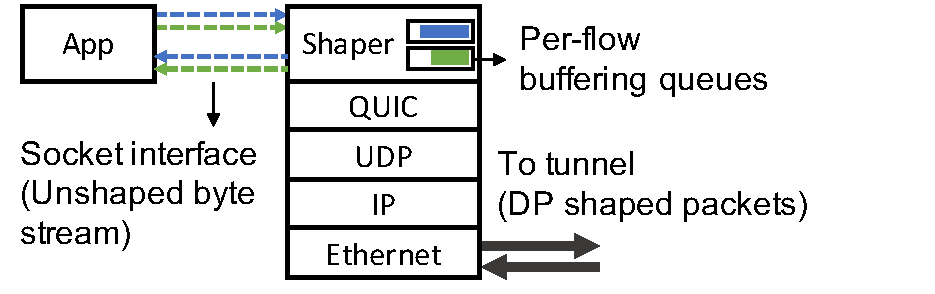
\includegraphics[width=\columnwidth]{figures/netshaper/tunnel-endpoint-design.pdf}
    \caption{Overview of tunnel design (one endpoint)}
    \label{fig:tunnel-endpoint-design}
\end{figure}

NetShaper adopts a transport-layer proxy tunnel architecture, where each end host application terminates the connection at its local tunnel endpoint (see \Cref{fig:netshaper-setup}). Hence, each communication byte stream traverses through three piecewise connections: (i) Between the application and the local tunnel endpoint, (ii) between the tunnel endpoints, and (iii) between the remote tunnel endpoint and the remote application.

\begin{figure}[!htb]
    \centering
    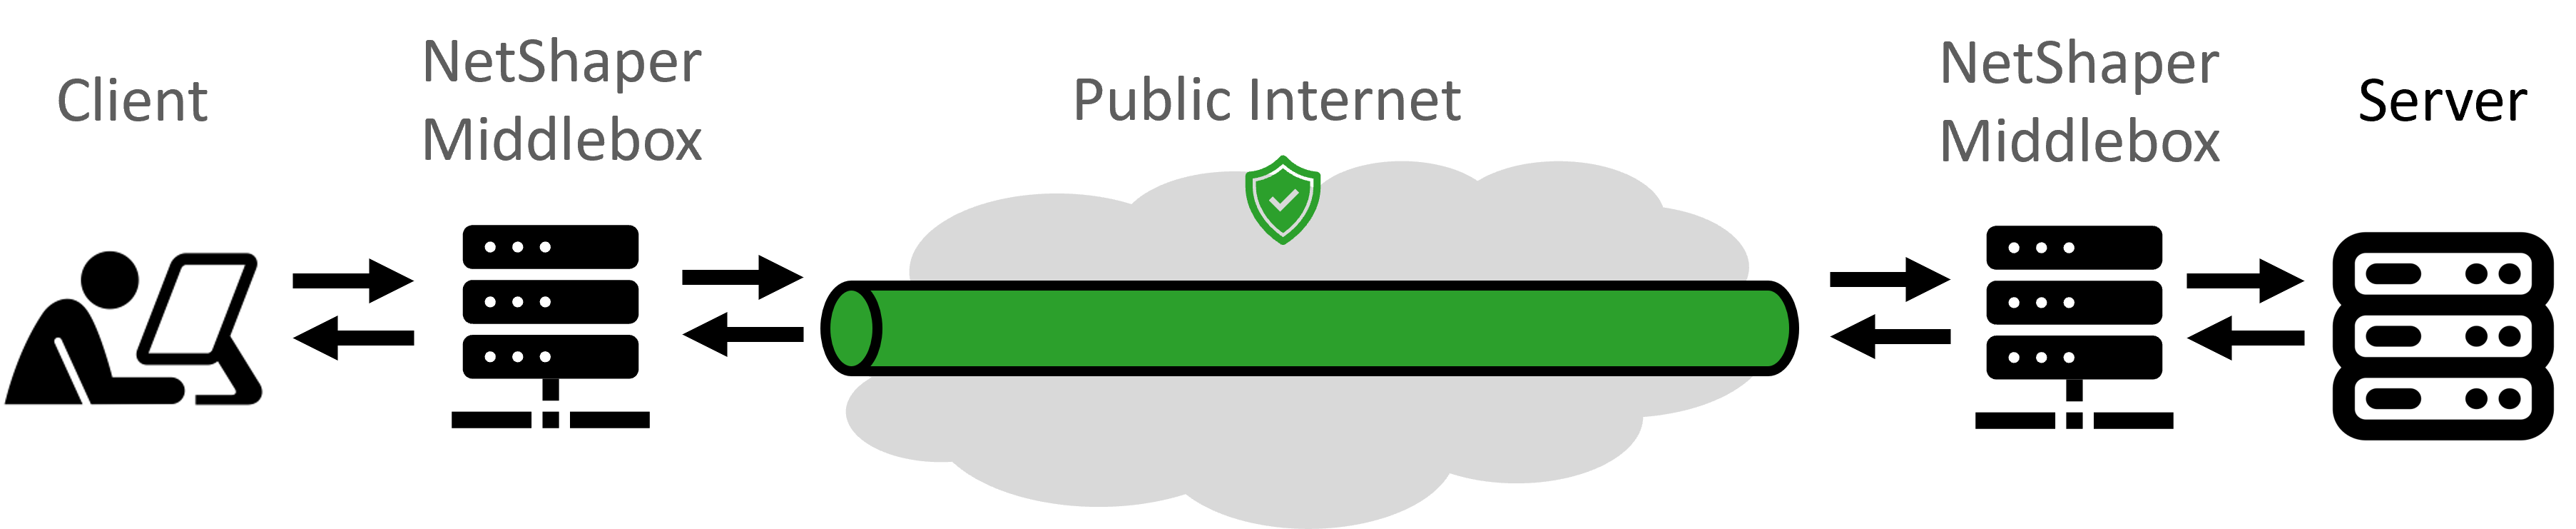
\includegraphics[width=\columnwidth]{figures/netshaper/netshaper-setup.png}
    \caption{NetShaper's Tunnel Setup}
    \label{fig:netshaper-setup}
\end{figure}

\paragraph{Scaling with multiple end hosts.}
In order to amortise the overhead and scale with multiple end hosts, the tunnel can rely on QUIC streams (see \Cref{subsec:netshaper-background-quic})
Using this, the tunnel can proxy the payload of multiple end hosts through a single QUIC connection between a pair of middleboxes.

While QUIC can support arbitrary initialisation and termination of streams, each stream has an associated header, which would increase the total transmission size.
For example, when transmitting $n$ bytes in a single stream, the total transmission size would be $n + S_{header}$.
However, when transmitting $k$ streams of $n/k$ byte each, the total transmission size would be $n + k*S_{header}$. 
An adversary may be able to distinguish between these two scenarios.
In order to avoid such a situation, the tunnel must initialise a fixed number of streams per QUIC connection during the setup phase, and not establish any more streams once the tunnel is established.


\subsection{Tunnel Operations}

\paragraph{Tunnel setup and teardown.}
In order to communicate securely using NetShaper's tunnel, the application first needs to send a configuration message to its local tunnel endpoint.
The configuration message contains the privacy parameters, the source and destination (IP and port), and a reliability flag determining whether the tunnel should provide reliable delivery semantics.
Next, the tunnel endpoint needs to establish a QUIC connection with the tunnel endpoint on the destination side and configure the privacy parameters for that connection
\footnote{A new connection may not be established if an existing connection with similar parameters offering similar or better privacy guarantees already exists.}.
The local tunnel endpoint also establishes three types of QUIC streams: control, data and dummy.
One \textit{control stream} is used to transmit messages regarding connection establishment or termination by an endpoint.
\textit{dummy stream} is used to transmit the dummy/padding whenever the DP query results in more bytes than available from the sending application
\footnote{We do not use QUIC's PADDING frames as they do not elicit acknowledgements, and hence, are distinguishable on the network \cite{quic_rfc}.}.
One or more \textit{data streams}, each carrying the data/payload of one application.

The tunnel is configured with an idle timeout, after which one endpoint initiates the termination sequence and shuts down the established QUIC streams and the QUIC connection.

\paragraph{End host connection establishment and termination.}
Once the tunnel setup is complete, the end host applications can establish or terminate connections with each other.
Whenever an end host application establishes a connection, the Shaper maps this connection to a QUIC \textit{data stream}.
It then transmits a message of connection establishment containing the source, the destination, and the ID of the associated \textit{data stream} on the \textit{control stream}.
The remote tunnel establishes a new connection to the remote application based on the connection establishment message and maps this connection to the relevant \textit{data stream}.
Similarly, whenever an end host terminates a connection, the Shaper transmits a connection termination message on the \textit{control stream}, and the remote end host terminates the connection with the remote application after ensuring all pending data has been transmitted.

\paragraph{Outbound traffic shaping.}
The Shaper accumulates the application byte streams in buffering queues.
At the start of every finite interval, the Shaper measures the total size of the available data in the buffering queues ($L$). 
It then adds some noise $\eta$ to this size based on the configured privacy (DP) parameters.
Hence, the total size to be transmitted in this window is $L + \eta$.
In the same interval, it also prepares the \textit{shaped buffer} that contains $R$ payload bytes and $D = max(0, L + \eta - R)$ dummy bytes and enqueues it for QUIC to transmit.
QUIC then takes this buffer and prepares QUIC packets based on the constraints on the connection (e.g. maximum transmission unit, congestion window size, and flow window size).
Then, QUIC sends these prepared packets out by using the networking stack's UDP layer.

\paragraph{Inbound traffic processing.}
For incoming shaped packets, QUIC sends an ACK to the sender and decrypts the packet.
The tunnel endpoint then processes the decrypted packet, drops the dummy bytes, and forwards the application data byte streams to the relevant remote applications.

\endinput
\section{Middlebox Implementation}
\label{sec:netshaper-middlebox-implementation}

While it is possible to apply NetShaper framework's approach at any network layer, we chose to develop the system as an L4 (Transport Layer) proxy.
This enables the system to be easily deployable, entirely in userspace and without requiring any superuser privileges. 
Developing NetShaper at L2 (Data Link Layer) or L3 (Network Layer) would require the deployer to either have the ability to modify the OS kernel or deploy some form of kernel bypass.

\begin{figure}[!htb]
    \centering
    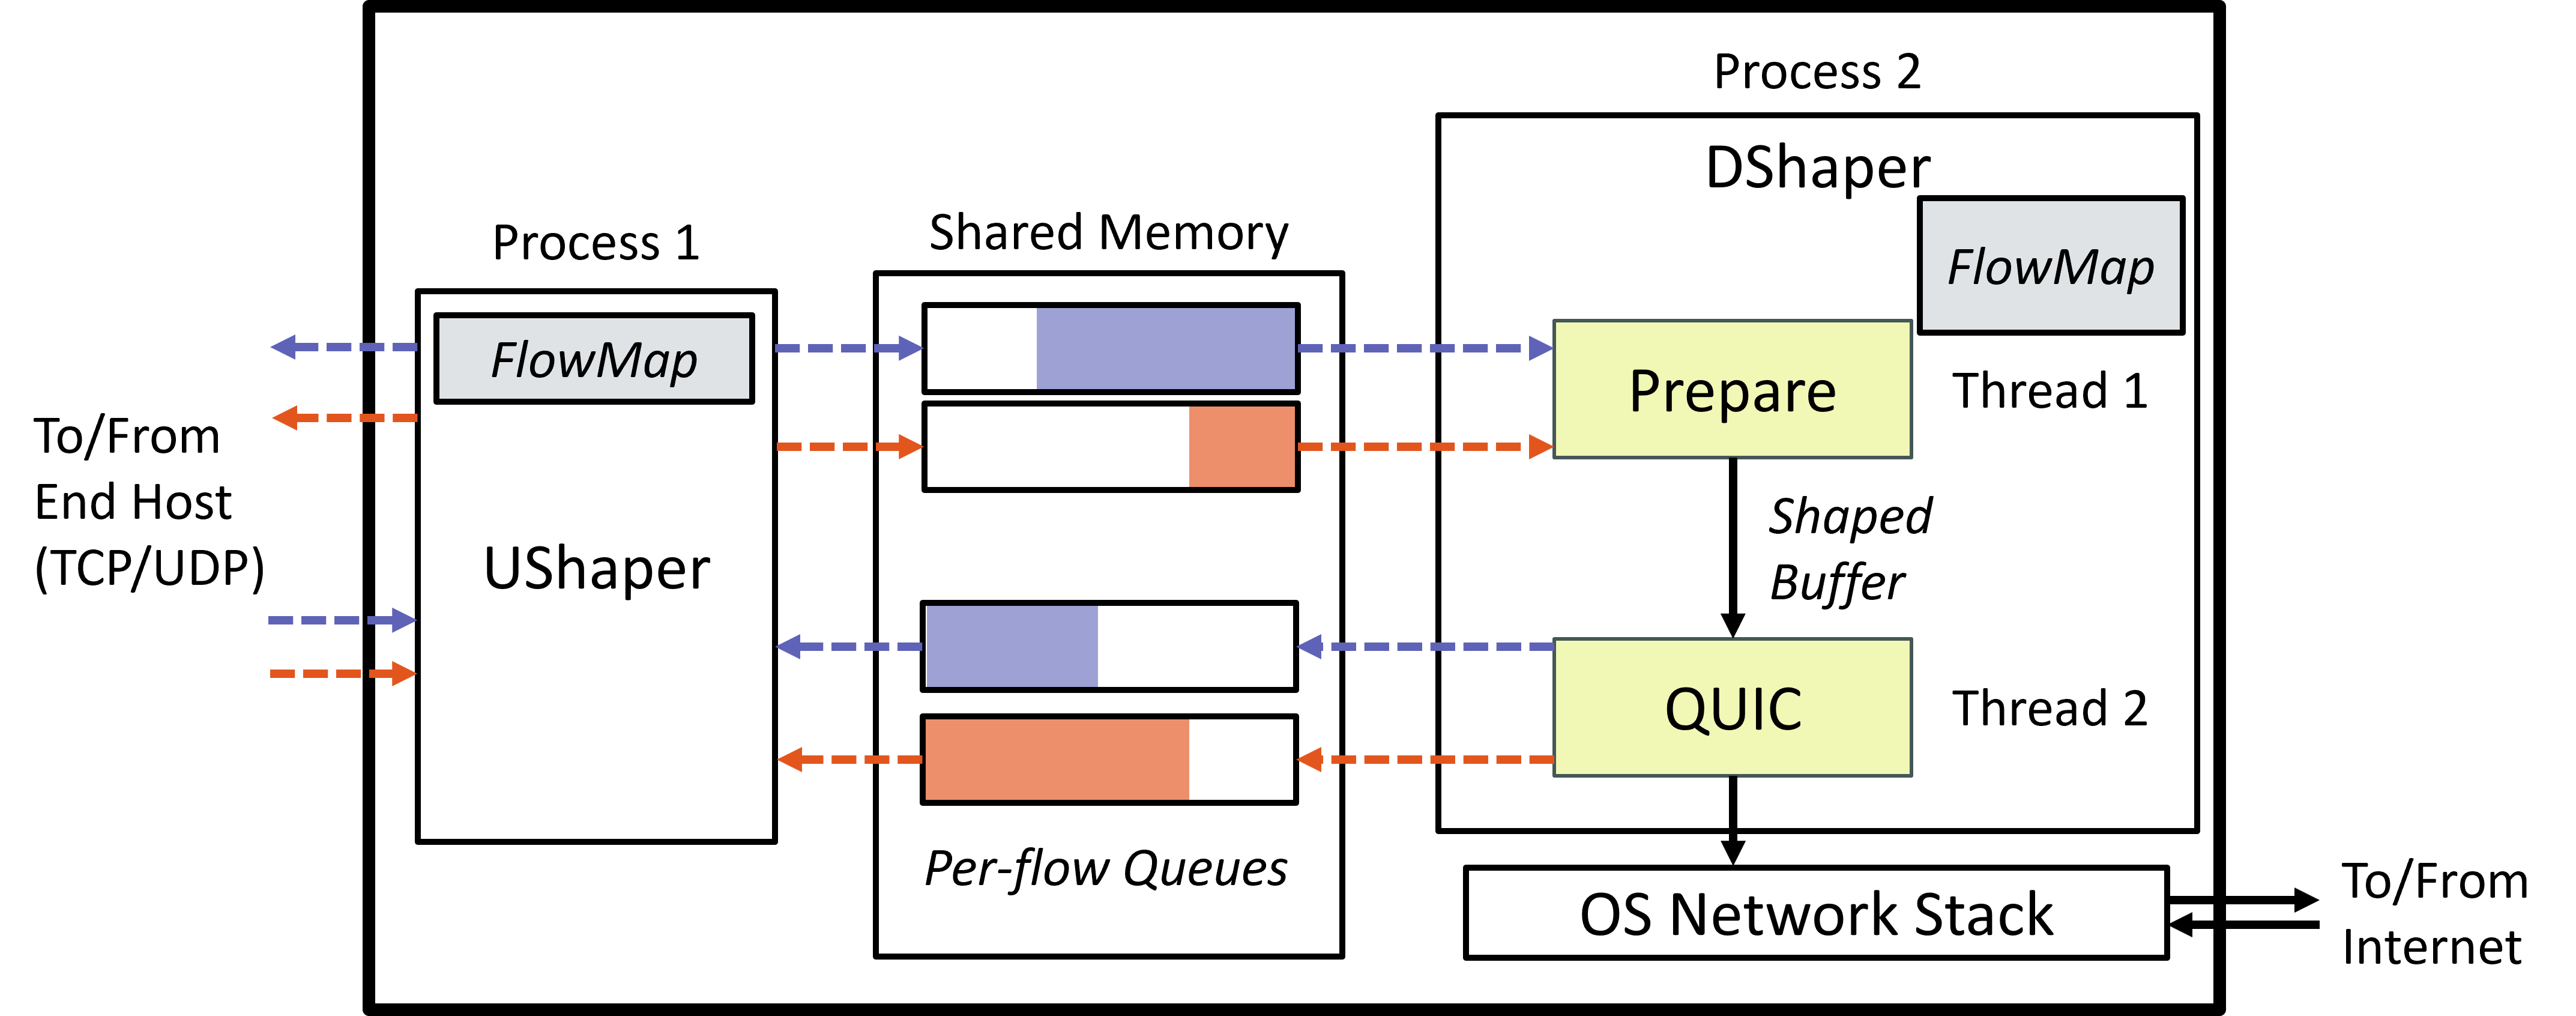
\includegraphics[width=\columnwidth]{figures/netshaper/middlebox-implementation.png}
    \caption{NetShaper Middlebox Implementation}
    \label{fig:middlebox-implementation}
\end{figure}

As outlined in \Cref{fig:middlebox-implementation}, NetShaper's middlebox consists of two main processes: \textit{UShaper} and \textit{DShaper}, and a shared memory between them.

\paragraph{Shared Memory.}
Both \textit{UShaper} and \textit{DShaper} have a shared memory between them.
The shared memory consists of $2*(k + 2)$ Lamport Queues (LQs) \cite{lamportqueue}
\footnote{Lamport Queues are lock-free single producer single consumer (SPSC) queues. They are useful to ensure that no locking is required when putting data in or pulling data out from the queues.}, 
where $k$ is the fixed number of \textit{data streams} that were configured at initialisation.
There is one queue for each direction of transmission for each of the $k$ streams that are initialised, and one for each of the \textit{control stream} and \textit{dummy stream}.

Similar to the stream types outlined in \Cref{sec:netshaper-designing-traffic-shaping-tunnel}, the \textit{control LQ} transmits the information about a connection establishment or termination by an end host application. 
The \textit{dummy LQ} carries dummy data that is received from or sent to the tunnel.
Each \textit{data LQ} carries the application byte stream that has been received from or has to be sent to the remote application.


\paragraph{UShaper.}
The \textit{UShaper} implements a client or a server to communicate with the end host.
The \textit{UShaper} also consists of a FlowMap 
\footnote{The NetShaper paper shows a shared FlowMap between the \textit{UShaper} and \textit{DShaper}. However, to avoid locking and signalling across processes, we improved the implementation to instead synchronise the FlowMap by using a \textit{control LQ} that is shared between the processes.}
that maps an end-host application with a corresponding pair of LQs.
\textit{UShaper} updates the FlowMap whenever an end-host application establishes or terminates a connection, and a \textit{control} message is generated and either sent or received on the \textit{control} LQ.
In addition, it assigns an unused pair of LQs (one outbound and one inbound) to a new client and revokes that whenever the client terminates the connection.
The \textit{UShaper} receives outbound traffic from the end host and enqueues the payload in the assigned LQ.
Similarly, it dequeues inbound traffic from the inbound LQs and sends it to the corresponding end hosts.
% We have implemented \textit{UShaper} in 1100 lines of C++ code.

\paragraph{DShaper.}
The \textit{DShaper} consists of two threads, \textit{Prepare} and \textit{QUIC worker}, and a FlowMap.
The FlowMap maps an LQ with a pre-initialised QUIC stream.
The \textit{Prepare} thread measures the data available in the outbound LQs at the start of the window $W$.
It then adds noise to this available size based on the DP parameters.
Finally, it enqueues the payload and padding that needs to be transmitted.
The \textit{QUIC worker} transmits the enqueued data out to the network.
It also processes the received data, places it in the relevant LQ, and updates the FlowMap when necessary.
% We have implemented \textit{DShaper} in 1800 lines of C++ code
% \footnote{\label{footnote:msquic-loc} Both \textit{UShaper} and \textit{DShaper} consist of the MSQUIC implementation of QUIC, which is 180k lines of code, and is a part of NetShaper's TCB.}.

\subsection{Ensuring secret-independent shaping}
\label{subsec:netshaper-secret-independent-shaping-implementation}

To enforce DP guarantees, \textit{DShaper} needs to transmit $L + \eta$ bytes in every finite interval $W$.
To achieve this, \textit{DShaper} should satisfy the following properties.
\textbf{P1}: The \textit{Prepare} thread should calculate $L + \eta$, prepare a buffer of that size, and enqueue that buffer for the \textit{QUIC worker} thread to transmit within $W$.
\textbf{P2}: The \textit{QUIC worker} thread should encrypt the packets from the buffer and forward them to the UDP stack, such that the total size of the payload prepared in $W$ is $L + \eta$.
\textbf{P3}: The UDP stack should transmit the encrypted packets within $W$.
Thanks to the post-processing property of DP, it suffices to only ensure P1, and \textbf{P4.} that the \textit{QUIC worker} thread prepares the QUIC packets independently of the secret data.

However, there are some challenges in satisfying P1 and P4.
As both the \textit{Prepare} thread and \textit{UShaper} deal with secret-dependent data, their execution time may affect the observable network behaviour, which in turn may lead to exposed secrets.
While the end host application is isolated from the middlebox, its flow control may be secret dependent and can affect the execution time of the \textit{Prepare} thread.
For example, the presence or absence of an application's traffic can affect the time it takes for the \textit{Prepare} thread to prepare the buffers.
If the \textit{QUIC worker} thread starts transmitting immediately, the secret dependent information may be visible in the network behaviour. 
This would also break P4, as the \textit{QUIC worker} thread prepares the QUIC packets based on the secret-dependent flow control.
NetShaper addresses this by ensuring that the \textit{Prepare} thread takes a fixed amount of time ($T_{prep}$) to prepare the shaped buffer.
Also, it locks the buffer when enqueuing it to the \textit{QUIC worker} so that the \textit{QUIC worker} does not start preparing the packets and transmitting them immediately.
The \textit{Prepare} thread releases the lock after a fixed amount of time $T_{enq}$.
As such, the \textit{QUIC worker} thread only receives the shaped buffer at regular intervals of time.
We empirically profile the time taken by the \textit{Prepare} thread for $T_{prep}$ and $T_{enq}$ for buffers of various lengths and set the values to the maximum observed, with an additional margin on top.
We have outlined pseudo-code for both the \textit{Prepare} thread and the \textit{QUIC worker} thread in \Cref{lst:prepare_and_worker}.


To ensure further isolation, the \textit{Prepare} and \textit{QUIC worker} threads are both run on separate physical cores.
\textit{UShaper} runs on a yet different core to ensure that the sending and receiving of unshaped, secret-dependent data does not affect the execution time of either of the \textit{DShaper} threads.
We assume that QUIC's encryption and decryption time correlates only with the shaped buffer's size, not its content.



\begin{minipage}{\textwidth}
\lstinputlisting[language=Python]{code/netshaper/prepare_and_worker.py}
\captionsetup{type=lstlisting}
\caption{Pseudo-code of the \textit{Prepare} and \textit{QUIC Worker} threads}
\label{lst:prepare_and_worker}
\end{minipage}

\section{Evaluation}
\label{sec:netshaper-evaluation}

We evaluate NetShaper on a variety of performance metrics.
First, we evaluate the peak line rate that NetShaper can support. 
Next, we evaluate the maximum throughput that the NetShaper middlebox can sustain.
Then, we measure the latency that NetShaper's middlebox will incur without any traffic shaping.
And finally, we measure the relation between NetShaper's latency and $W$ when traffic is being shaped.

\subsection{Setup}
\label{subsec:netshaper-evaluation-setup}

\begin{figure}[!htb]
    \centering
    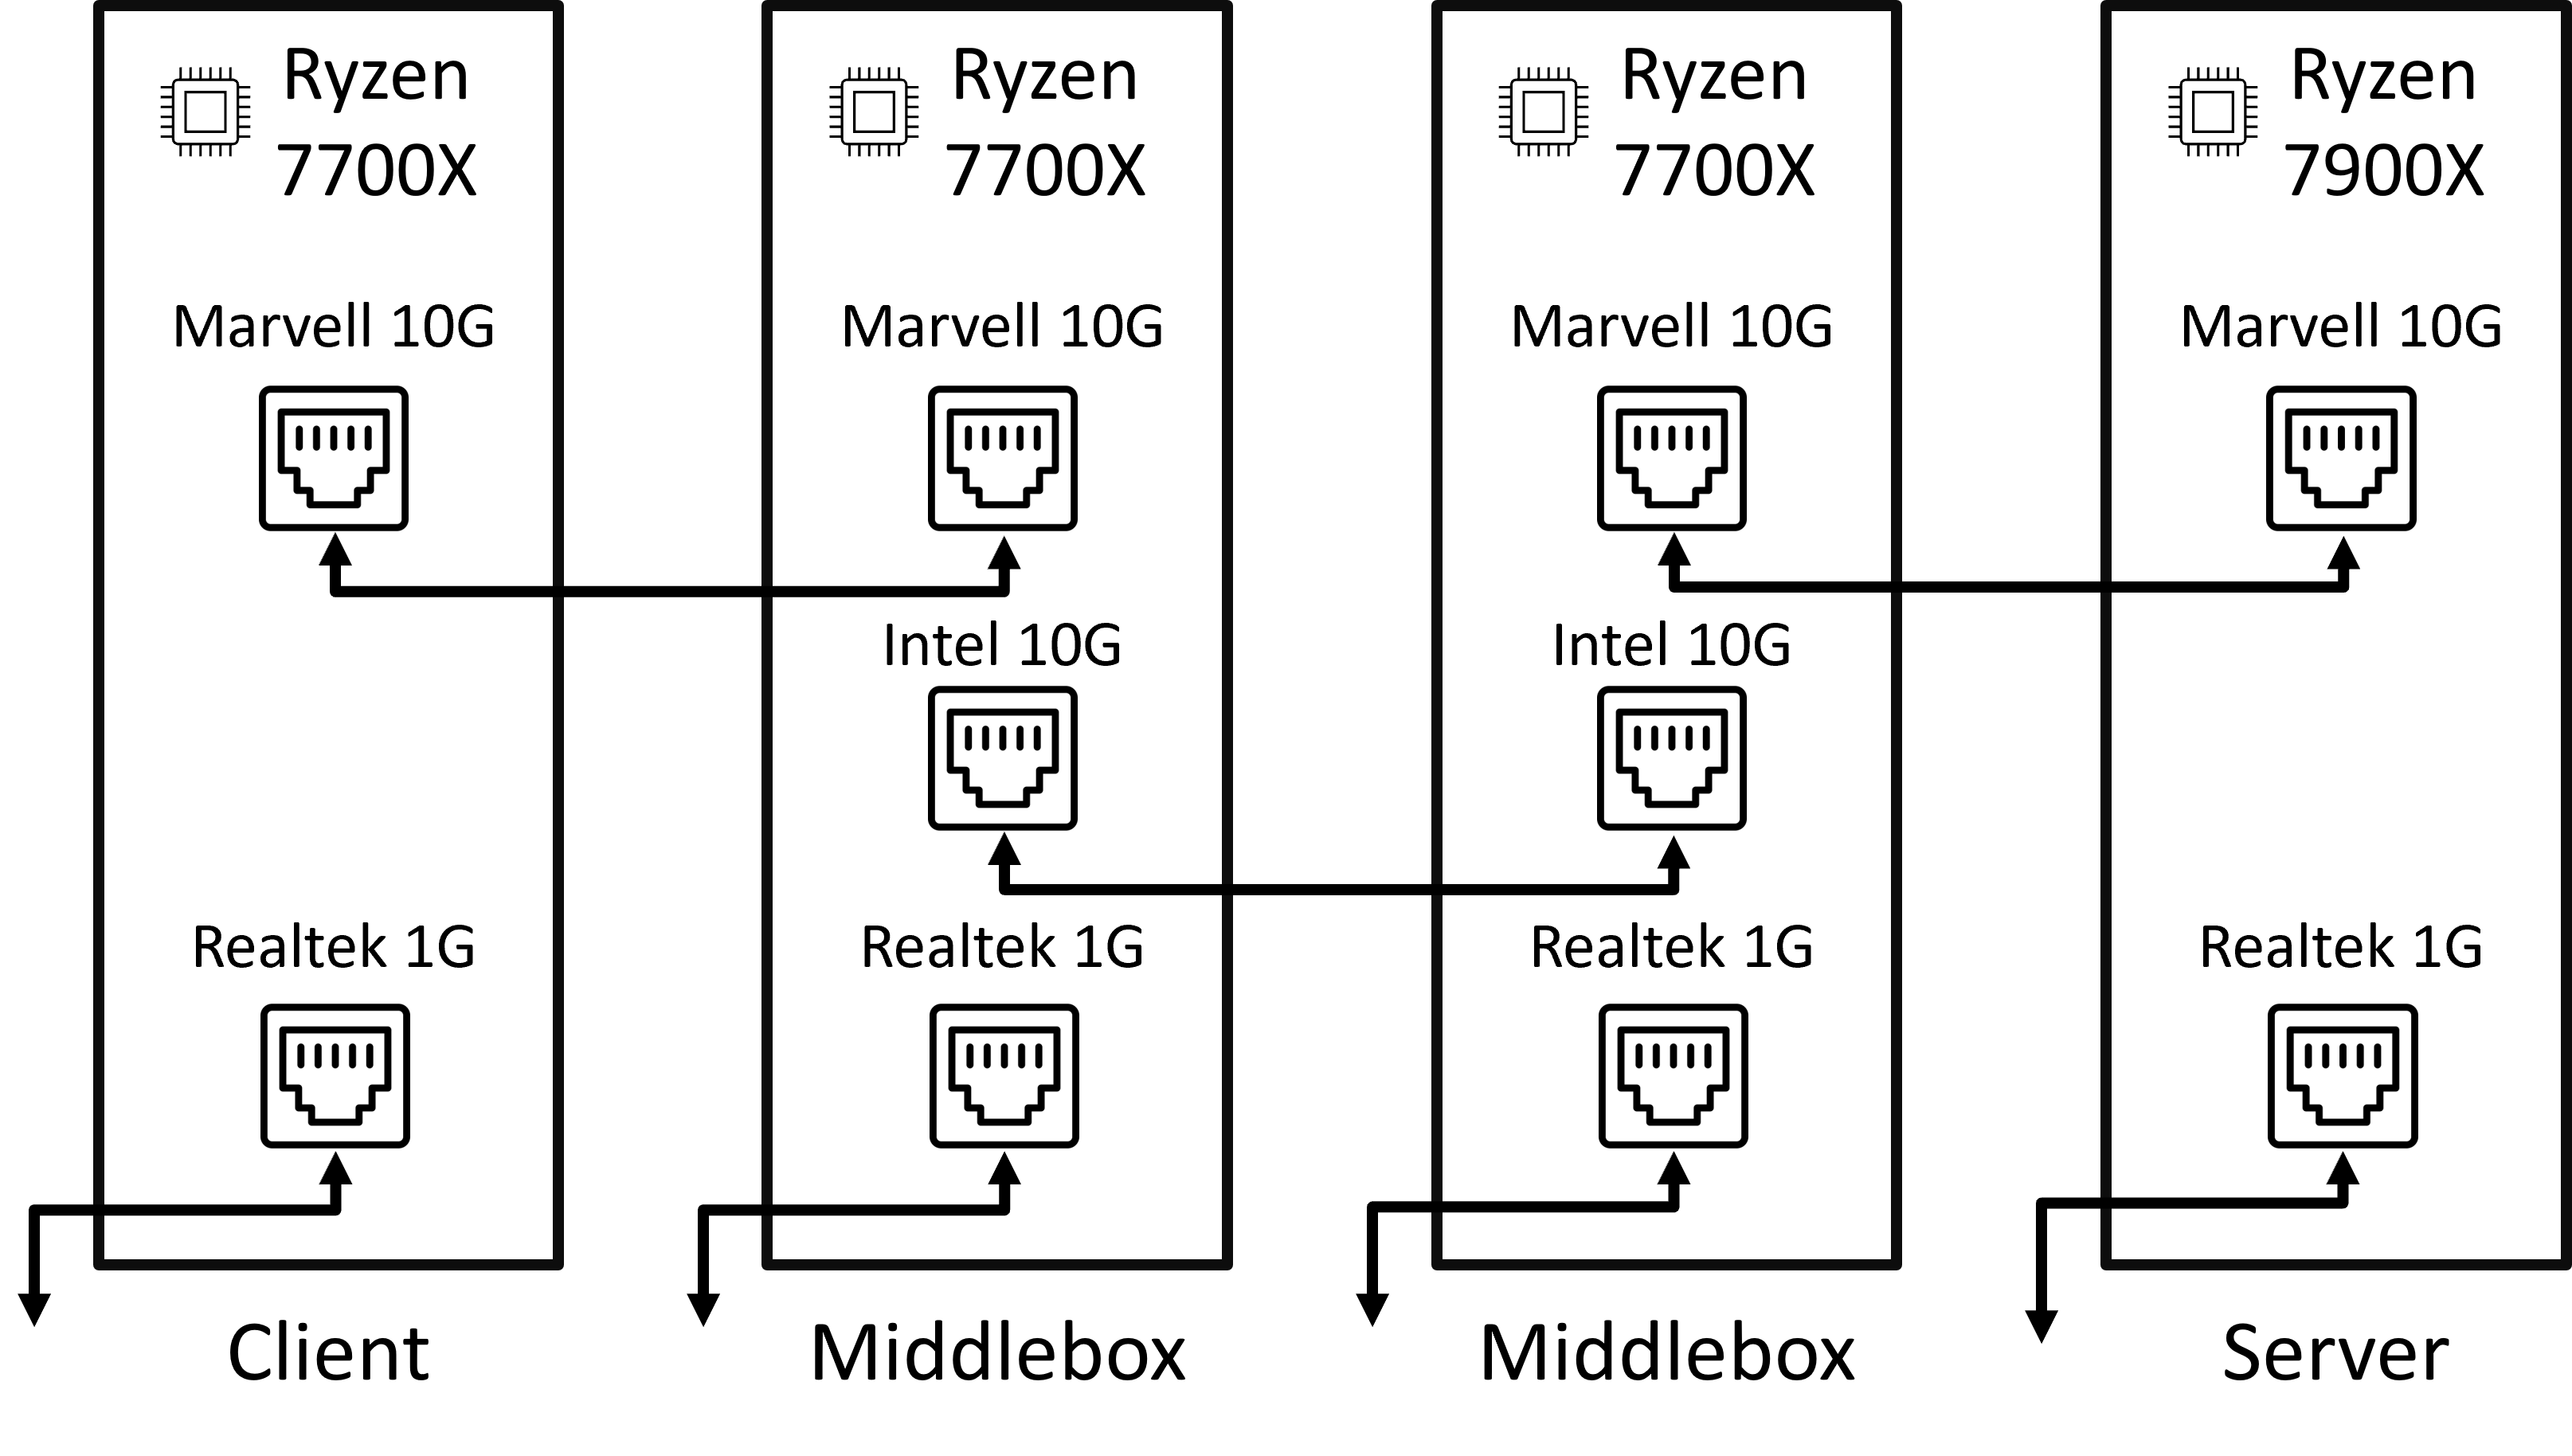
\includegraphics[width=\columnwidth]{figures/netshaper/testbed-setup.png}
    \caption{Evaluation Setup}
    \label{fig:testbed-setup}
\end{figure}

Our setup consists of four desktops, each of which consists of 32GB RAM, 1TB storage, one Marvell AQC113CS-B1-C 10G NIC, and one Realtek RTL8111 1G NIC.
We use the Realtek NIC only as a management NIC and do not run any experiments on it.
Three of the desktops have an AMD Ryzen 7 7700X processor, and one has a more powerful AMD Ryzen 9 7900X processor, which we use as the server.
The middleboxes are connected to each out via an additional Intel X550-T2 10G NIC.
The client and the server are connected to their local middleboxes via the Marvell 10G NIC.
This forms a linear topology, as outlined in \Cref{fig:testbed-setup}
All the desktops run Ubuntu 22.04.02 (linux kernel version 5.19)

All of our experiments contain a baseline setup (\textbf{Base}) wherein the client is directly connected to the server via the Marvell 10G NIC, bypassing the middleboxes.

\begin{comment}

Mention iperf, wrk2 (modified), nginx?
Maybe here maybe in the experiments themselves

\end{comment}
\subsection{max \#packets}
\label{subsec:netshaper-evaluation-max-packets}
\subsection{max throughput}
\label{subsec:netshaper-evaluation-max-throughput}
% \subsection{minimum DShaper loop duration}
\label{subsec:netshaper-evaluation-minimum-dshaper-loop-duration}
\subsection{impact of dshaper loop duration}
\label{subsec:netshaper-evaluation-impact-of-dshaper-loop-duration}
\section{Limitations}
\label{sec:netshaper-limitations}

Our implementation has two security limitations.
First, it relies on the MSQUIC implementation of QUIC, which utilises OpenSSL, which may not provide constant time cryptography.
However, this limitation can be easily remedied by modifying MSQUIC so that it uses a constant-time cryptography library such as WolfSSL \cite{wolfssl}.
Second, it is difficult to profile for $T_{prep}$ and $T_{enq}$. 
If the time taken by the \textit{Prepare} thread exceeds that of the profiled values, it violates our theoretical DP guarantees. 
However, in practice, it is difficult to exploit these violations for carrying out traffic analysis based network side-channel attacks.

NetShaper has two more limitations in terms of usability and performance.
First, we currently require a custom configuration format supplied by the client to configure the destination for a connection. 
However, given the modular architecture of our system, one can easily implement \textit{UShaper} as a SOCKS5 proxy \cite{leech1996socks} or any other standard proxy protocol.
Second, the current implementation dedicates only one core each to \textit{UShaper}, \textit{Prepare}, and \textit{QUIC Worker}. These can become a bottleneck. 
While it is relatively simple to dedicate more cores for \textit{UShaper} or \textit{QUIC Worker}, doing so for the \textit{Prepare} thread is non-trivial, as it has to aggregate data from all the available clients.
\section{Related Work}
\label{sec:netshaper-related-work}

While prior work has explored various approaches for mitigating network side-channel attacks, most focus on conceptual methods, with only a few providing a practical system to address the issue.
CS-BuFLO \cite{cai2014csbuflo} applies traffic shaping by transmitting a fixed number of bytes at semi-regular intervals while remaining receptive to congestion control.
DeltaShaper \cite{barradas2017deltashaper} obfuscates the traffic shape to always look like a video conference stream.
It transcodes the application traffic as a video stream that is then fed to Skype with a virtual camera.
While both implementations require modifications to the end hosts, their approach can conceptually be implemented as a middlebox.
However, their approach is not adaptive to the application traffic and, hence, can result in either high bandwidth overhead or high latency.
In addition, DeltaShaper is also unable to support more than one application stream at a time.
HTTPOS \cite{luo2011httpos}, ALPaCA and LLaMA \cite{cherubin2017llama}, and Walkie-Talkie \cite{wang2017walkie} all require modification of the end-hosts and support only HTTP applications.

Pacer \cite{mehta2022pacer} provides a shaping tunnel that is conceptually similar to NetShaper's tunnel design (see \Cref{sec:netshaper-designing-traffic-shaping-tunnel}).
However, Pacer protects a cloud tenant's data from being leaked to a co-located adversary via congestion in a shared network link.
As such, Pacer controls the transmit time of TCP packets based on the shaping schedule and congestion control signals.
Achieving this requires non-trivial modifications to the end-hosts.
On the other hand, NetShaper protects applications in different private networks that are communicating over the public internet. 
As such, NetShaper can be placed as a gateway for the private networks to access the public internet, thus requiring none to minimal changes on the end-hosts.
In addition, NetShaper's approach requires precise timing only for the generation of bursts of DP length and not for the actual network transmission, requiring no modification of the underlying network stack.

QCSD \cite{smith2022qcsd} shares similarities with NetShaper, as both rely on the QUIC protocol. 
However, QCSD requires modifications to the client-side browser, unlike NetShaper. 
Since no server-side modifications are necessary, QCSD depends on the client to control the amount of data sent by the server, including the addition of padding or dummy bytes.
This approach requires the client to be aware of the sizes of the content the server hosts, as otherwise, the client may request more padding/dummy bytes than the requested content contains.
In addition, their approach does not scale well with an increasing number of client applications, as each client application will require its own QUIC connection, which in turn results in per-client dummy/padding bytes being transferred.

Ditto \cite{meier2022ditto} and NetShaper both shape traffic at network nodes that do not coincide with the end-hosts.
However, NetShaper's approach is hardware-independent, modular, and portable.
As such, NetShaper can be integrated into routers, gateways, end-hosts, and even programmable switches such as the one on which Ditto was deployed.


% \chapter{Side Channels in Interconnects}
\label{ch:interconnect-sc}

\section{Introduction}
\label{sec:interconnect-sc-introduction}
\section{Background}
\label{sec:interconnect-sc-background}

\subsection{PCIe}
\label{subsec:interconnect-sc-background-pcie}
\subsection{CPU Architecture}
\label{subsec:interconnect-sc-background-cpu-arch}

Modern CPUs have many components, including execution units, caches, PCIe root complex, and DRAM controllers.
Some subset of these components is always traversed when data is sent to or from the CPU to the PCIe endpoints.
The behaviour of each component may impact how the side-channel attack is carried out.
As such, it becomes necessary to understand all the components involved in a PCIe transaction.

\begin{figure}[!htb]
    \centering
    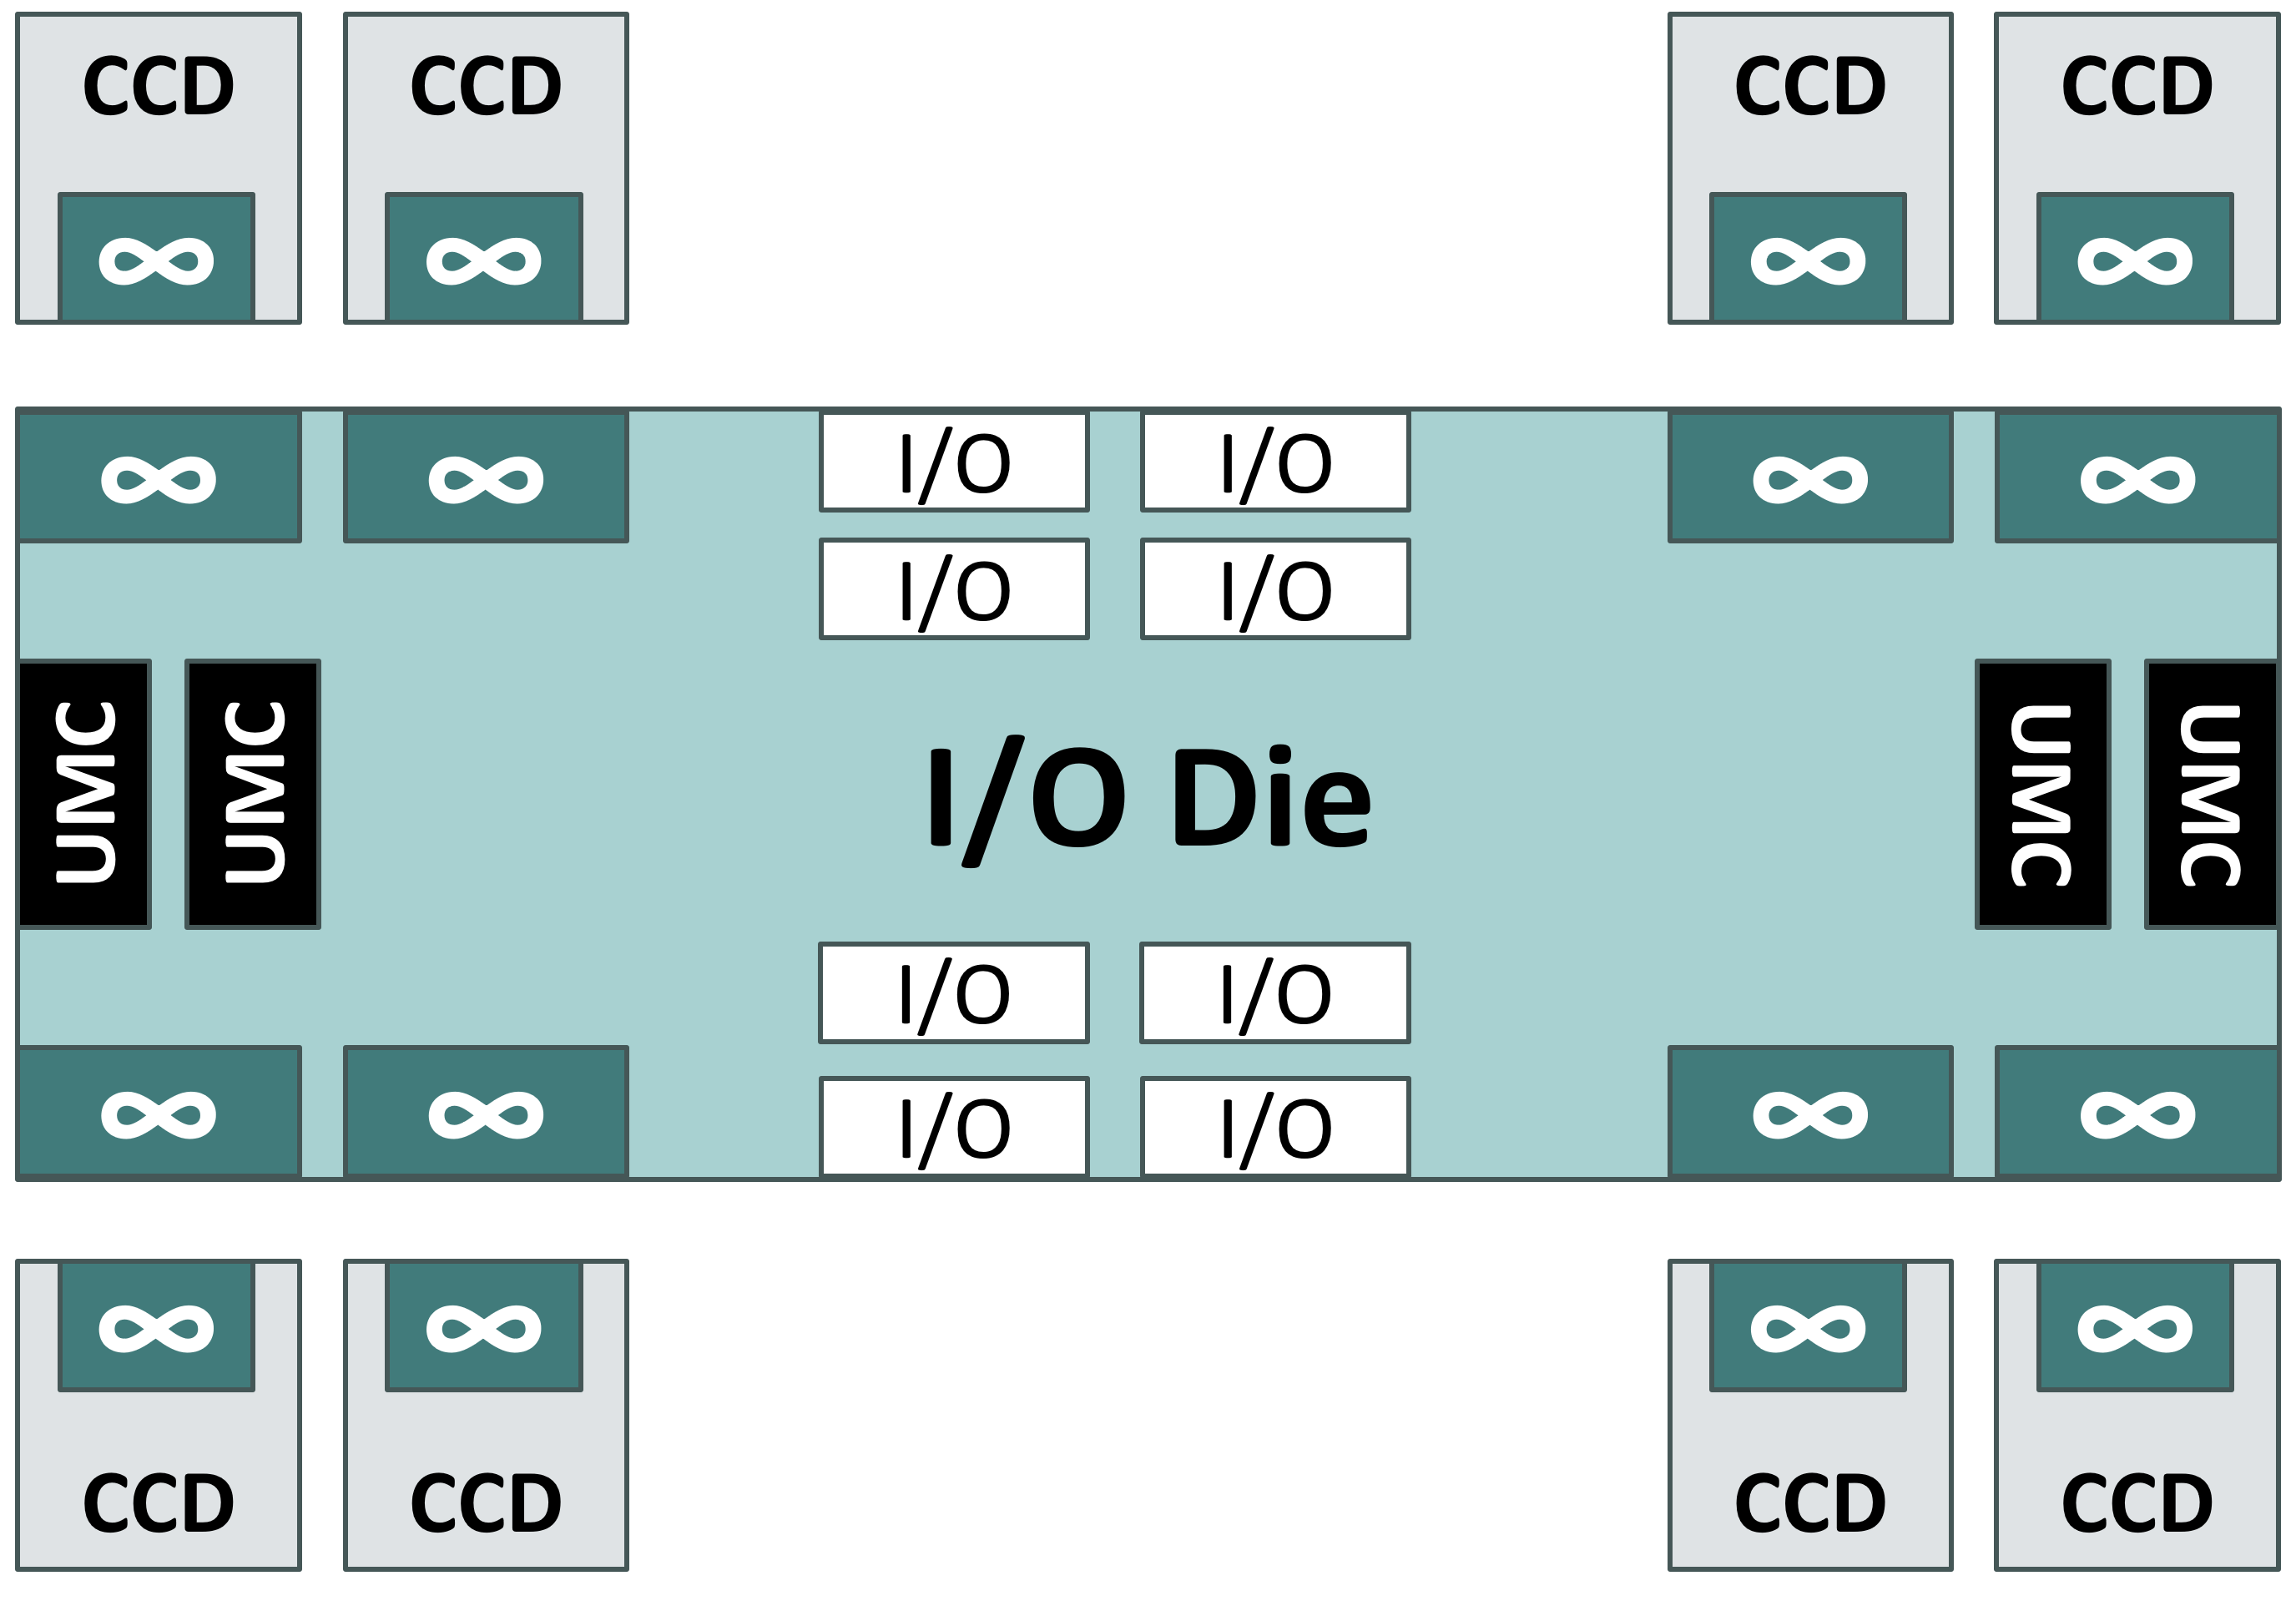
\includegraphics[width=\columnwidth]{figures/interconnect-sc/amd_arch/processor.png}
    \caption{AMD EPYC Zen 3 Architecture - CPU}
    \label{fig:amd-cpu}
\end{figure}


\Cref{fig:amd-cpu} shows a high-level overview of the architecture of the AMD EPYC Zen 3 processors.
The figure shows the following components:
\textbf{1) I/O:} The component that handles the input-output from the peripheral devices. This is where the PCIe communication happens.
\textbf{2) UMC:} The Unified Memory Controller is the controller that communicates with the DRAM.
\textbf{3) CCD:} The Core Complex Dies are where the cores (execution units) and caches reside.
\textbf{4) Infinity Fabric ($\infty$):} The interconnect that connects all of the components within the AMD CPU.

\subsubsection{CPU Pipelines}
\label{subsubsec:interconnect-sc-background-cpu-arch-pipelines}

Modern CPUs rely on executing multiple instructions simultaneously to maximise performance.
To achieve this, the CPUs have a multi-stage pipeline with the following stages: 1) Fetch, 2) Decode, 3) Schedule and Execute, and 4) Retire.
We provide a simplified view of the pipeline in the CPU cores of the AMD EPYC Zen 3 processors in \Cref{fig:amd-core} and a brief description of each of the stages below:\\
\textbf{Fetch: } This stage fetches the next macro-op from the cache or the memory. 
However, the next macro-op to be fetched may not be deterministic, given the program may contain branches. 
In such cases, this stage also uses branch prediction to speculate on which instruction may be executed next and fetch that instruction.\\
\textbf{Decode: } This stage involved decoding the fetched macro-op into one or more micro-ops, which are then forwarded to the next stages.\\
\textbf{Schedule and Execute: } The scheduler(s) determine which instruction can be executed next based on the availability of the data that the instruction requires. 
This ensures that a long-running instruction (e.g., where the data is unavailable) does not stall all other independent instructions that can be executed.
As such, instructions here can be executed out of program order. 
Once the instruction has finished execution and the output (if any) is available in the registers, the instruction is removed from the scheduler.
As load and store are common but time-consuming instructions, this stage also consists of a load-store queue where pending load and store operations are held. \\
% \footnote{In Zen 3 cores, the load/store unit has a capacity of 72 loads and 64 stores.}. \\
\textbf{Retire: } This stage ensures that instructions are retired in the program order so that the program can remain oblivious to the out-of-order execution that occurred in the previous stage.

\begin{figure}[!htb]
    \centering
    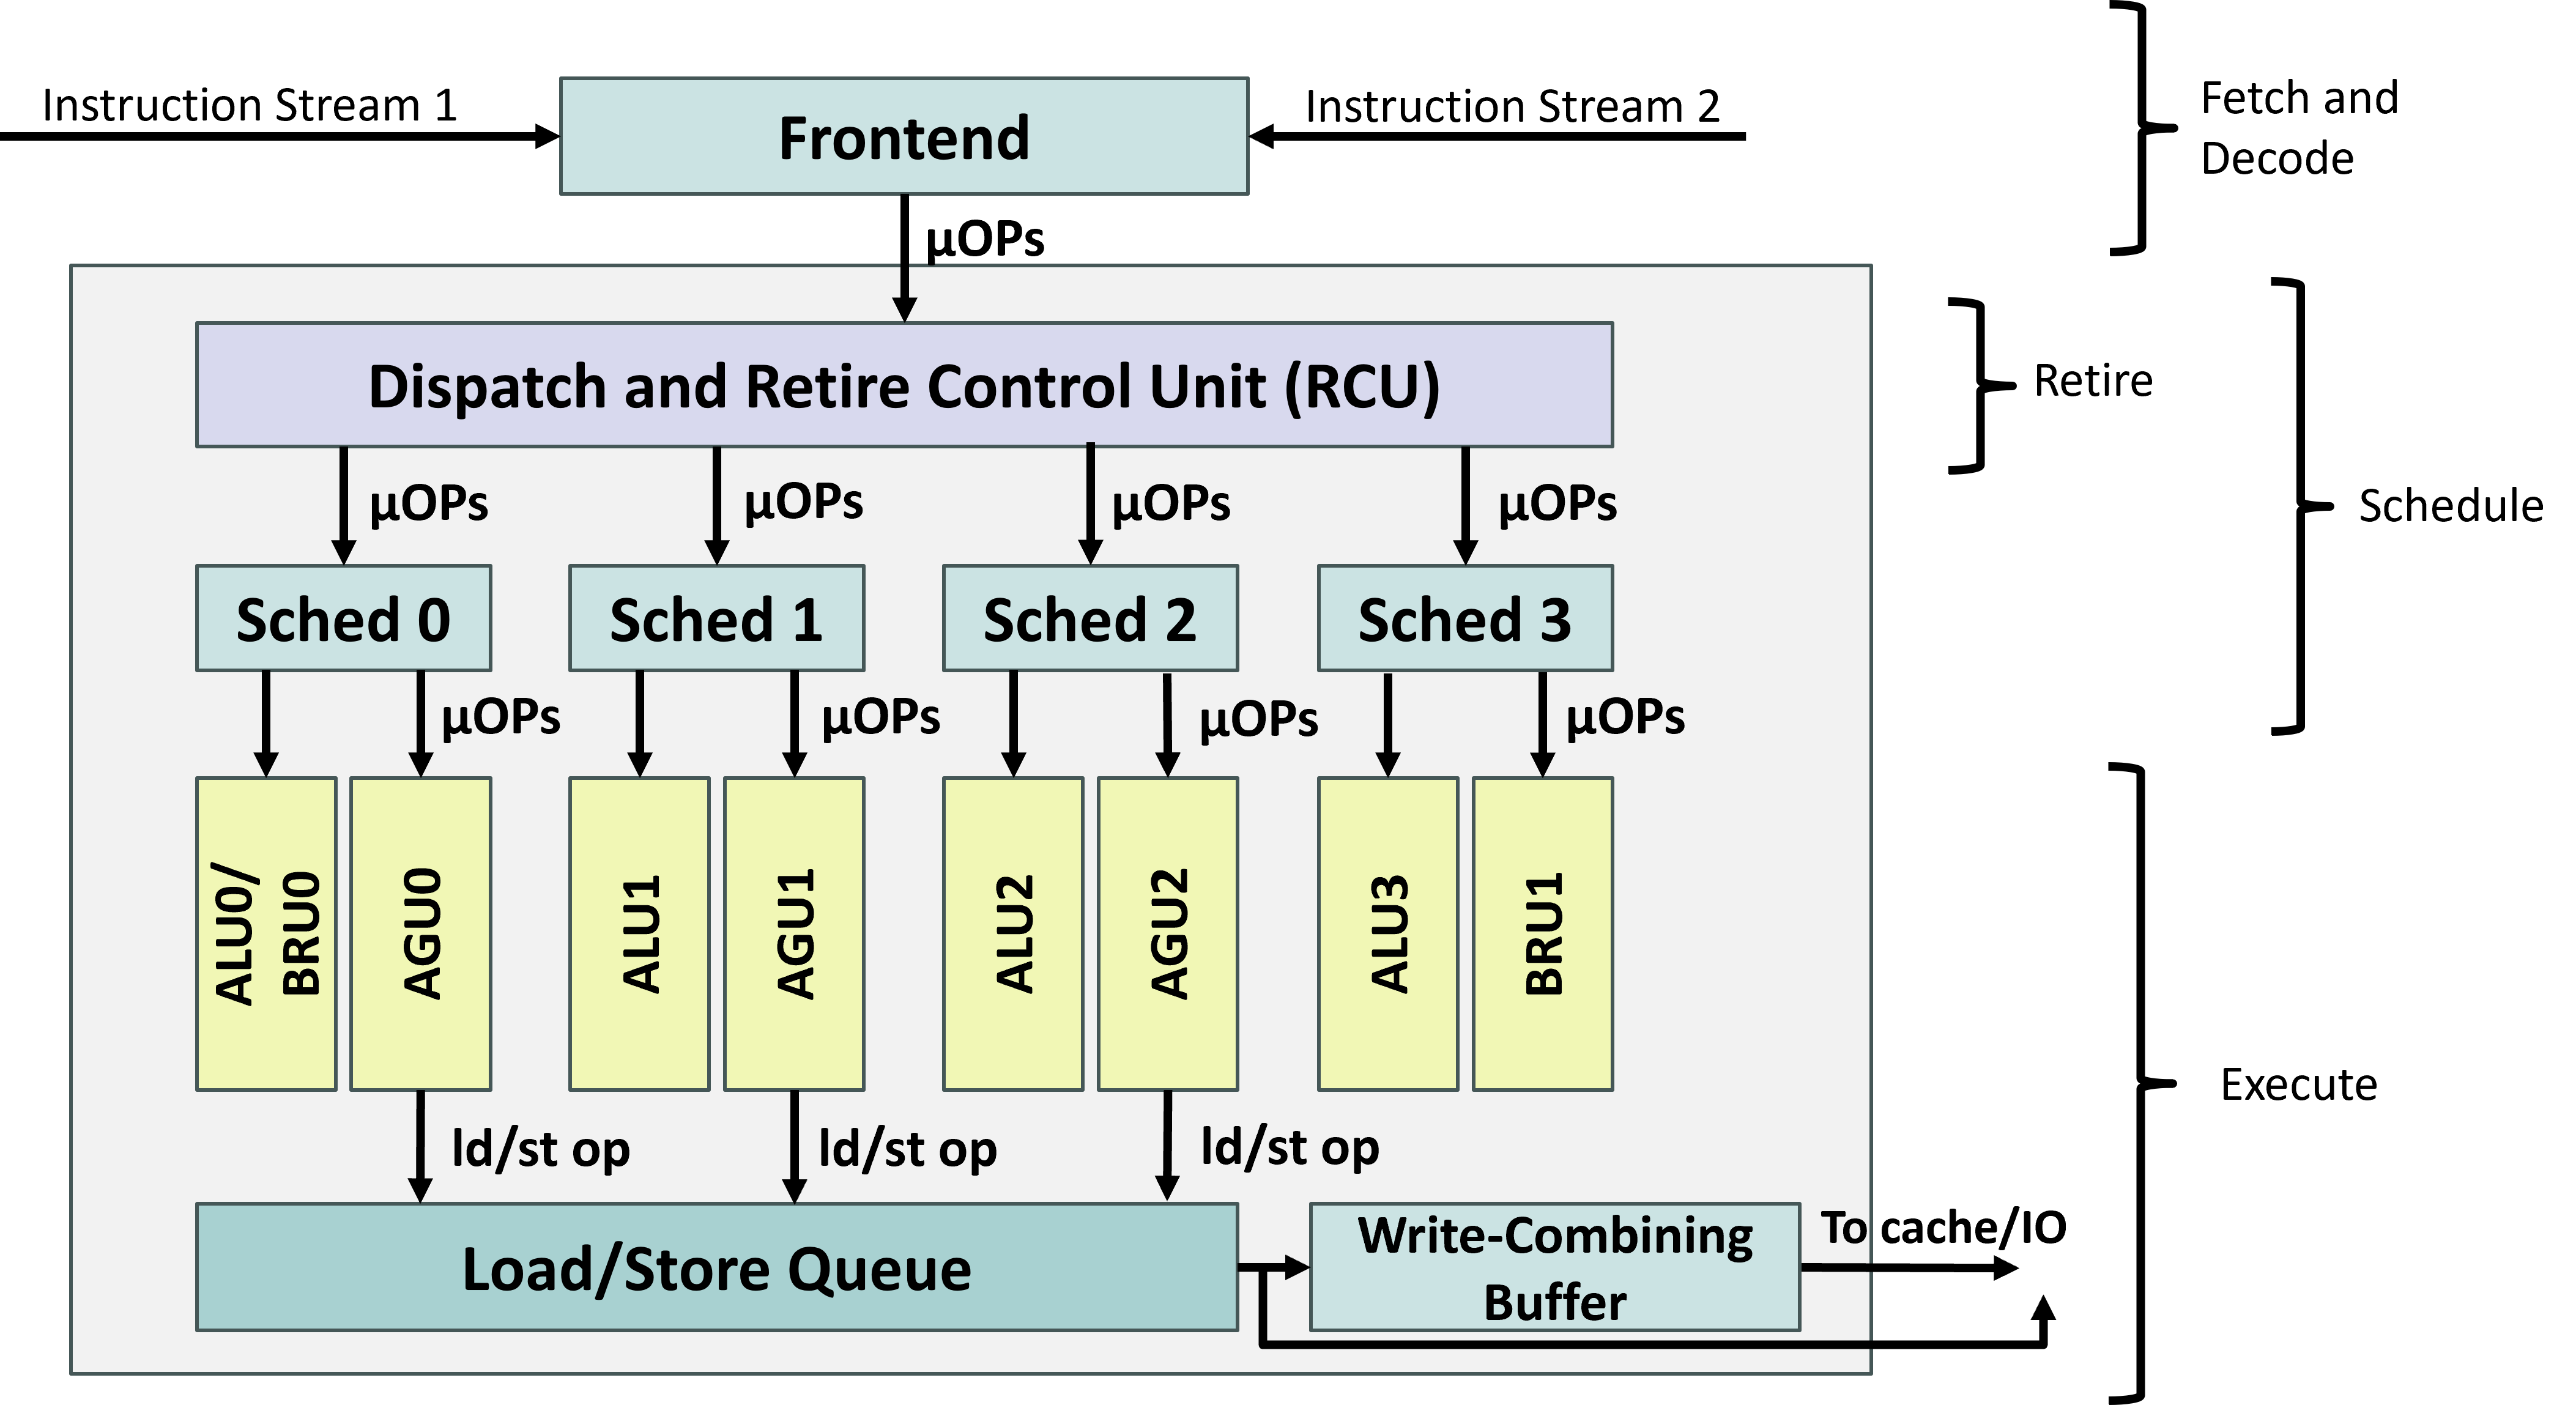
\includegraphics[width=\columnwidth]{figures/interconnect-sc/amd_arch/core.png}
    \caption{AMD EPYC Zen 3 Architecture - Core}
    \label{fig:amd-core}
\end{figure}

\subsubsection{PCIe transactions to/from CPU}
\label{subsubsec:interconnect-sc-background-cpu-arch-pcie-transactions}

A program running on the CPU can transfer data to the PCIe device/endpoint in two significant ways: 1) Memory operations via memory-mapped IO (MMIO) and 2) Direct memory access (DMA).
MMIO enables the CPU to map some memory region of the PCIe endpoint in the CPU's physical address space.
Any process with the proper permissions can then map this memory within the process and perform normal \textit{load} or \textit{store} operations on this memory.
However, this approach requires the execution units of the CPU to issue repeated \textit{load/store} instructions to copy data to the PCIe endpoint.
While this method is helpful for reading or writing limited content, such as small configuration parameters, to the PCIe endpoints, it is inefficient for transferring a large amount of data.
To alleviate this, many PCIe endpoints have a unique hardware component called a direct memory access (DMA) controller.
The DMA controller is purpose-built to copy large chunks of contiguous data without involving the execution units of the CPU.

For MMIO-based transactions, the load or store instructions go through the same instruction pipeline outlined in \Cref{fig:amd-core}. 
From the Load Store Queue, they enter the I/O die shown in \Cref{fig:amd-cpu} and exit through the I/O block to the connected PCIe endpoint.
For DMA transactions, which are typically initiated by the PCIe endpoint, the transaction enters the I/O block. 
After address and protocol translations, they are transmitted to the DRAM through the UMC.
\subsection{Side Channels in Interconnects}
\label{subsec:interconnect-sc-background-side-channels}

Conceptually, a side-channel attack in interconnects is similar to a side-channel attack in internet networks. 
The attacker creates congestion on a buffer in the communication path between the host (CPU) and the peripheral (e.g., GPU), such as the Rx/Tx buffers in the transaction layer implementation of the PCIe controller (see \Cref{fig:pcie-controller}).
The attacker then observes the delay in transmitting their traffic.
This delay will be proportional to the data the victim transfers, which would help the attacker gain insight into the victim's traffic shape.

However, a few differences between interconnects and traditional networks make it challenging to implement such an attack in interconnects.

First, the bandwidth of interconnects such as PCIe are at least an order of magnitude higher than that of internet networks.
While a typical bandwidth in an internet network is between 0.125 - 1.25 GBps 
\footnote{Internet network bandwidth is typically measured in bits per second, while for interconnects, it is measured in bytes per second. Typical internet bandwidth is 1-10 Gbits per second.},
PCIe 4.0 can operate at a rate of 32GBps.
The high bandwidth makes it difficult to saturate the PCIe link.

Second, latency in PCIe is at least three orders of magnitude smaller than that of internet networks.
Typically, internet latency is measured in milliseconds, while PCIe latency is measured in hundreds of nanoseconds to microseconds.
The low latency makes it difficult for the attacker to measure the delays accurately.

Third, unlike internet networks, PCIe does not extend outside the machine of the host CPU.
This further adds to the challenge that the attacker needs to co-locate with the victim application on the same machine.

Fourth, the PCIe protocol has a fixed behaviour depending on the type of transaction.
The attacker can not craft their own packets and can not change how the hardware issues the PCIe transactions.
% Most transaction types can not generate enough traffic to even come close to saturating the bandwidth of PCIe. 
% While saturating the bandwidth may not be necessary to create a side-channel attack, it would be useful if there is always at least one attacker packet in the buffer whenever the victim might transmit.
% This would ensure that the attacker can observe a delay in their own packets for each packet or set of packets the victim transmits.


Nevertheless, prior work demonstrated that an adversary can create congestion in the PCIe links by saturating the PCIe bandwidth.
Using this congestion, the adversary can determine which website a user is visiting \cite{tan2021invisible, side2022lockeddown}, what the user is typing in a GUI environment \cite{tan2021invisible}, what machine learning model they are training \cite{tan2021invisible}, or what resources they are using on an FPGA connected via PCIe \cite{giechaskiel2022cross}.
Recent work also shows that congestion in PCIe can be used as a covert channel to exfiltrate data \cite{giechaskiel2022cross, khaliq2021timing}.

\begin{comment}
https://www.linkedin.com/pulse/pci-express-primer-3-transaction-layer-simon-southwell/
\end{comment}
\section{Threat Model}
\label{sec:interconnect-sc-threat-model}
\section{Setup}
\label{sec:interconnect-sc-setup}

Our setup consists of a single server with two NUMA sockets, each consisting of an AMD EPYC 7343 processor with 16 physical cores.
The server also has an Nvidia A100 GPU with 80GB HBM2e memory.
The GPU is directly connected to the CPU in the first NUMA socket (i.e., without any PCIe switch being involved).

We use the CPU in the first NUMA socket only for all the experiments.
We also isolate the cores we run the experiments on from the Linux kernel and divert as many system processes and interrupts to other cores as possible
\footnote{We isolate the cores using \textit{isolcpus} option during boot. We also use \textit{cpuset} and \textit{irqbalance} to move system processes and interrupt handling to cores not used for the experiment.}.
We fix the CPU core frequencies at 2.3 GHz to ensure that changing core frequencies do not impact our experiments.

\section{Generating contention via CPU instructions}
\label{sec:interconnect-sc-store-ops}

There are two major ways one can generate traffic on the PCIe link: 
1) CPU load/store instructions on memory-mapped PCIe device memory, I/O or configuration address space, and 
2) Direct memory access (DMA) to copy data between the PCIe device memory and the DRAM.
In this section, we discuss how to use CPU instructions to generate the traffic and defer the discussion of generating traffic via DMA to \Cref{sec:interconnect-sc-dma}.

An adversary can generate traffic from the CPU by mapping a PCIe device resource to an application running on the CPU and issuing load or store operations on the mapped memory.
Each load/store operation will be buffered in the PCIe controller until a transaction layer packet (TLP) is generated and ready to be transmitted.
The actual transmission time of the packet is influenced by two factors:
1) The ordering of the packets, as outlined in \Cref{tab:pcie-transaction-ordering-rules}, and
2) The number of pending packets that are not subject to any ordering rules relative to the current packet.
If the packets do not have any relative ordering rule, it is reasonable to assume that the controller follows a simple first come, first serve policy.
As such, any packet generated by the adversary can either be delayed due to the presence of existing traffic in the buffer or not be delayed, as there is no traffic in the buffer.
This allows the attacker to observe the presence or absence of victim traffic without necessarily saturating the PCIe bandwidth.


To observe the victim traffic, the attacker always needs to have at least one packet pending in the PCIe controller, which can be delayed by the presence of the victim traffic.
The attacker also needs to ensure that the packet can not be delayed because of their own traffic.
To achieve these goals, the attacker needs to determine the correct combination of the PCIe resource and instruction, as different instructions on different resources can lead to different PCIe transactions and transaction ordering rules.


\subsection{Challenges}
\label{subsec:interconnect-sc-store-ops-challenges}


\subsubsection{Determining the right PCIe resource and instruction combination}

Of the transaction types outlined in \Cref{tab:pcie-transaction-types}, a software application can generate only configuration read and write and memory read and write on a modern system that only has PCIe devices
\footnote{I/O reads and writes may be available if a legacy PCI device is attached.
The software application does not control messages and Completions and, hence, can not be generated directly by the adversary.}.
However, as memory reads, configuration reads, and configuration writes are all non-posted transactions, they all exhibit the same behaviour.
As such, exploring only memory reads suffices for exploring all non-posted transactions.
Similarly, exploring memory writes as transactions that an attacker can use suffices to explore all posted transactions. 


To profile the execution time of memory \textit{load} and \textit{store} instructions, we use a program that follows the pseudocode outlined in \Cref{lst:pcie-mem-reads-v-writes}.
As we can see in \Cref{fig:pcie-mem-reads-v-writes}, the execution time of memory loads (and consequently, non-posted transactions) increases linearly with the number of memory loads issued.
Each \textit{load} instruction takes about 2000 cycles, which is 625ns on a processor with a base clock of 3.2GHz.
Most of the 625ns latency is composed of PCIe transfer time \cite{neugebauer2018understanding}, because a \textit{load} operation has to wait for a previous \textit{load} operation to complete 
\footnote{While this is not enforced by PCIe ordering rules, it may be enforced by the proprietary PCIe controller implementation.}.
Since each \textit{load} instruction must wait for the previous one to complete, the attacker cannot guarantee a packet is always ready in the PCIe controller for transmission when the victim is simultaneously transmitting.
However, a memory store does not have to wait for a previous store to complete.
As such, we determine that memory stores are the correct type of transaction for the attacker.


\begin{minipage}{\textwidth}
    \lstinputlisting[language=Python]{code/interconnect-sc/pcie-mem-reads-v-writes.py}
    \captionsetup{type=lstlisting}
    \caption{Profiling the execution time of \textit{load/store} instruction.
    Each instruction reads/writes 8 bytes and is issued on a memory address at an offset of 64 bytes from the previous address.}
    \label{lst:pcie-mem-reads-v-writes}
\end{minipage}

\begin{figure}[!htb]
    \centering
    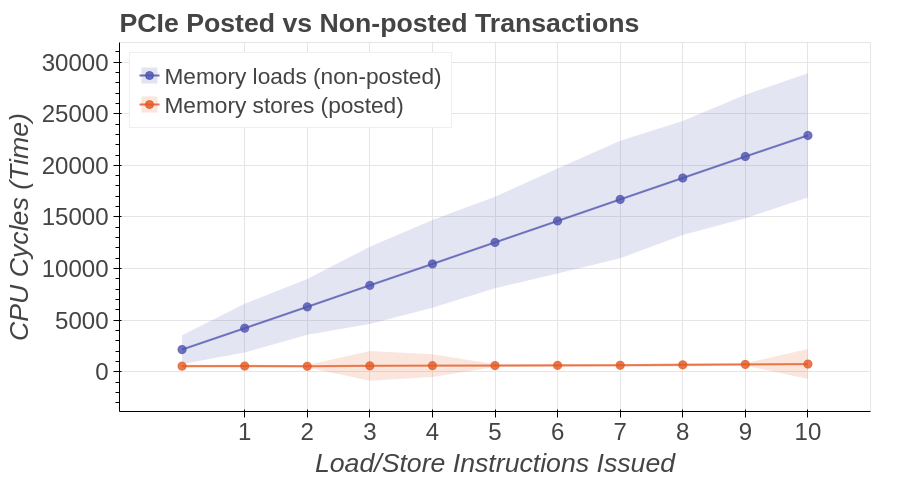
\includegraphics[width=0.8\columnwidth]{figures/interconnect-sc/store-ops/pcie_mem_reads_v_writes.png}
    \caption{Comparison: PCIe memory reads vs writes.
    The time is for completing all \textit{N} loads and stores.
    Each load needs to wait for the previous load to complete, but stores can be issued in parallel.}
    \label{fig:pcie-mem-reads-v-writes}
    % 2025-03-01_15-15
\end{figure}

\subsubsection{Issuing and timing a continuous stream of \textit{store} instructions}
\label{subsubsec:interconnect-sc-store-ops-challenges-measuring-time}

The \textit{mfence} instruction in \Cref{lst:pcie-mem-reads-v-writes} ensures prior \textit{store} operations complete before the \textit{mfence} does.
However, it disrupts the attacker from issuing a continuous stream of \textit{store} operations.
Simply removing the \textit{mfence} from the code is not sufficient, as then the end \textit{timer} may execute out of order with respect to the issued \textit{store} operations, giving a false execution time.
To fix this, the attacker needs a mechanism that can issue as many \textit{store} instructions as possible while having the ability to time the completions at the level of each instruction.

To measure the completion time of a \textit{store} operation which is issued out-of-order, we make use of two key insights:

\textit{First}, the CPU core needs to keep track of all instructions executed out-of-order so that they are retired in program order.
Keeping track of this requires a scheduler and a buffer in the hardware, which would have a limited and fixed size.
The AMD CPU has four schedulers as described in \Cref{subsubsec:interconnect-sc-background-cpu-arch-pipelines}. Each scheduler has a fixed number of instruction slots, $size_{sched}$
\footnote{AMD Zen 3 schedulers have $\sim$22-24 slots per scheduler \cite{gast2023squip}.}.
In addition, for tracking \textit{load} and \textit{store} operations that are in flight, the CPU also has a load-store queue (LSQ), with a fixed number of slots for loads ($size_{ldq} = 72$) and for stores ($size_{stq} = 64$) \cite{amd_7003_software_optimization_guide}.
Suppose the total number of pending (in flight) \textit{store} instructions is larger than the total size of the scheduler slots and the store queue. 
In that case, the next instruction will be blocked until one (or more) of the previous instructions finishes.
\textit{Second}, as the \textit{store} instructions may be executed out of program order, the attacker needs to observe the completion of the first \textit{store} instruction that was executed and not the first one by program order.
% As discussed in \Cref{subsec:interconnect-sc-background-cpu-arch}, each scheduler on the CPU core can hold 24 instructions.
% Any instruction not yet in the scheduler can not be executed out of order until it gets a slot in one of the schedulers.
% We leverage this CPU behaviour to develop a mechanism that can issue multiple \textit{store} instructions while having the ability to time individual completions.

We can use these insights to queue a \textit{timer} instruction immediately after issuing $size_{sched} + size_{stq}$ stores, and that \textit{timer} will execute only after the first \textit{store} instruction that was issued has been completed.
To achieve this, we need to ensure that we can issue $N = 3 * size_{sched} + size_{stq}$ 
\footnote{Only three schedulers have an address generation unit (AGU) that triggers \textit{load/store} operations.}
\textit{store} instructions in $t_{cpu} < 600~cycles$ (see \Cref{fig:pcie-mem-reads-v-writes}), to ensure that the CPU pipeline is filled before the first \textit{store} instruction retires.
As the AMD CPU can issue 2 \textit{store} instructions per cycle \cite{amd_7003_software_optimization_guide}, $t_{cpu} = N/2$.
For $size_{sched} = 24$ and $size_{stq} = 64$, $t_{cpu} = 68~cycles$.
As such, $t_{cpu}$ is well below the time taken for one store to complete and, hence, is sufficient to keep the CPU pipeline full.
% \footnote{Hence, if $size_{sched} = 24$, $N = 3 * 24 + 64 = 136$, and $t_{cpu} = N/2 = 68~cycles$.}.

Now, after the initial $N$ stores, if we issue a continuous stream of (\textit{timer}...\textit{store}) pairs, the \textit{timer} from the pair will be executed only after a previous \textit{store} retires.
As this \textit{timer} instruction will be executed immediately (out of order with the other stores), the \textit{store} in this pair will almost immediately occupy the now available scheduler slot, blocking the next \textit{timer}.
Thus, the difference in the results of the two \textit{timer} instructions reflects the variation in retirement times of consecutive \textit{store} instructions.
As the retirement times of the \textit{store} instructions are impacted by the PCIe transaction time, the attacker can use this mechanism to determine the presence or absence of victim traffic on PCIe.
We measure the time taken for various values of $N$ using the pseudo-code in \Cref{lst:measuring-time}
As we can see in \Cref{fig:measuring-store-time}, the measured time difference significantly increases after $N = 81$, validating this approach.

% However, we also observe that after $N = 81$, the stores retire in groups of $8$ instead of retiring individually.
% This can be an effect of some write-combining feature of the hardware.
% While the AMD CPU has a write-combining buffer immediately after the LSU, we explicitly rely on a PCIe resource marked as non-write-combining by Linux, which should prevent the hardware from relying on this buffer.


\begin{figure}[!htb]
    \centering
    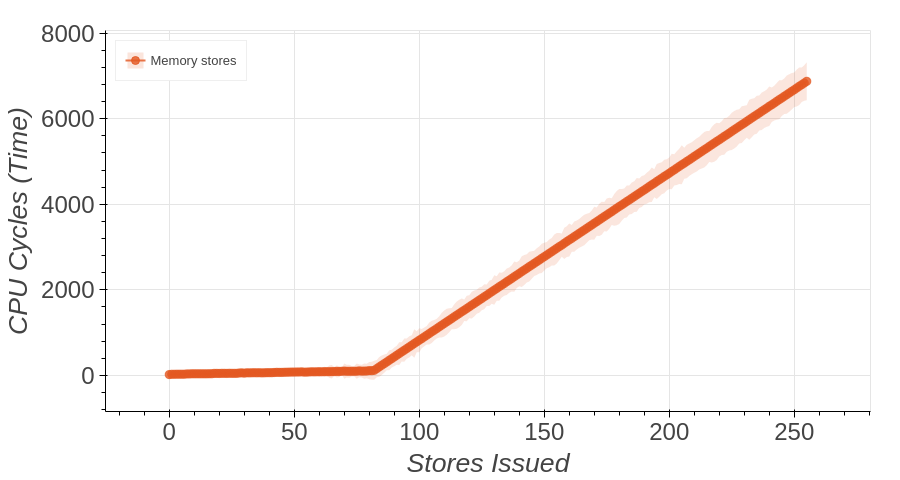
\includegraphics[width=\columnwidth]{figures/interconnect-sc/store-ops/measuring_store_time.png}
    \caption{Using head-of-line blocking in CPU pipeline to measure completion time of asynchronous stores.
    The timer is not executed out of order after a threshold number of \textit{store} instructions.}
    \label{fig:measuring-store-time}
    % 2025-03-04_15-28
\end{figure}

\begin{minipage}{\textwidth}
\lstinputlisting[language=Python]{code/interconnect-sc/measuring-time.py}
\captionsetup{type=lstlisting}
\caption{Pseudo-code for measuring time of individual stores while issuing multiple stores in parallel}
\label{lst:measuring-time}
\end{minipage}

\subsubsection{Microcode Updates}
\label{subsubsec:interconnect-sc-store-ops-challenges-microcode-updates}
However, the CPU behaviour observed in \Cref{fig:measuring-store-time} depends on the microcode the CPU is running.
The CPU microcode can change how the CPU behaves.
For example, the microcode can change how the schedulers schedule the instructions out of order, how the LSU tracks the stores in flight, or how the write-combining buffers combine multiple \textit{store} instructions to use the interconnects efficiently.

The results in \Cref{fig:measuring-store-time} are based on the microcode patch 0x0A0011D5 (for AMD EPYC 3rd gen 19h B1 processors) released on May 03, 2024 to address CVE-2023-31315 \cite{amd_microcode_update}.
Before this update (i.e. microcode patch 0x0a0011d3), the results were as shown in \Cref{fig:measuring-store-time-before-microcode-update}.
Here, $N = 120$, instead of $N = 80$. 
In addition, after the threshold of $N$, the stores complete in groups of $8$ instead of retiring individually.
This may be caused by unexpected behaviour of the write-combining (WC) buffers present after the LSU in the CPU pipeline.
The usage of the WC buffers also explains the high variation in the execution time measured, as the WC buffer combines writes based on specific threshold differences between the target addresses \cite{amd_7003_software_optimization_guide}, which are dependent on the order in which the stores were issued.
While we ensure that Linux marks the PCIe resource as a memory type that does not allow write-combining, the CPU may still use these buffers unexpectedly.
However, AMD does not offer changelogs for their microcode.
Hence, we cannot confirm what CPU behaviour changed between the given versions.


\begin{figure}[!htb]
    \centering
    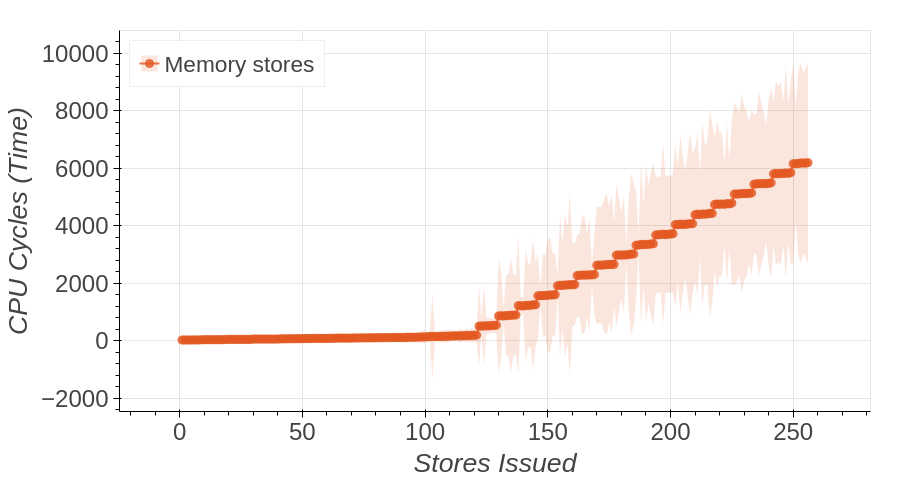
\includegraphics[width=\columnwidth]{figures/interconnect-sc/store-ops/measuring_store_time_before_microcode_update.png}
    \caption{Using head-of-line blocking in CPU pipeline to measure completion time of asynchronous stores.
    The timer is not executed out of order after a threshold number of \textit{store} instructions.}
    \label{fig:measuring-store-time-before-microcode-update}
    % 2024-10-12_18-07
\end{figure}

% \subsubsection{Reverse Engineering the CPU architecture}
% \label{subsubsec:interconnect-sc-store-ops-challenges-reverse-engineering}
\subsection{Using \textit{store} operations to observe presence/absence of victim traffic on PCIe}
\label{subsec:interconnect-sc-store-ops-measuring-time}
Now, we have a mechanism to issue multiple \textit{store} instructions in parallel while timing the completion of an individual (or a small group of) \textit{store} instructions.
We can use this mechanism along with the threshold of $N = 81$ to observe the presence or absence of victim traffic in the PCIe controller.
To achieve this, we execute the pseudo-code outlined in \Cref{lst:timing-victim-with-stores} while the victim transfers a large amount of data to or from the GPU via DMA
\footnote{Since most GPU-based applications rely on the DMA controller for efficient transfers, we assume that the victim uses DMA.}.

To evaluate our ability to detect victim traffic, we run the adversary for $10^5$ iterations.
At the same time, we execute the victim, which repeatedly (for $10^4$ iterations) performs a DMA transfer of either 4KB or 4MB.
The 4KB transfer does not saturate the PCIe link, while the 4MB transfer saturates the PCIe link (see \Cref{fig:bw-util-and-time-per-size}).
Additionally, we synchronise the execution of the critical code sections responsible for data transfers between the victim and the adversary. 
This synchronisation allows us to measure whether we can detect the presence or absence of victim traffic, even though such perfect alignment is unrealistic for a side-channel attack.

As shown in \Cref{fig:cpu-store-victim-observation}, the execution time of the individual \textit{store} operations by the adversary increases in the presence of victim traffic, irrespective of whether the victim is saturating the PCIe link or not.
In the absence of a victim, the \textit{store} instruction takes $<15~cycles$ to complete. However, in the presence of victim traffic, the execution time increases to $>15~cycles$ and drops down again once the victim is done transmitting.
As such, an adversary is able to determine the presence/absence of victim traffic.
The adversary observes a fixed delay in the execution time of the \textit{store} instruction irrespective of the size being transferred.
However, the duration for which the adversary observes the delay increases with the amount of data the victim transfers.
This is the case because the victim transfers the data using \textit{burst mode} of transfer, where the burst size is fixed.


\begin{minipage}{\textwidth}
    \lstinputlisting[language=Python]{code/interconnect-sc/timing-victim-with-stores.py}
    \captionsetup{type=lstlisting}
    \caption{Attacker code to detect presence of victim traffic via \textit{store} instructions}
    \label{lst:timing-victim-with-stores}
\end{minipage}

\begin{figure}[!htb]
    \centering
    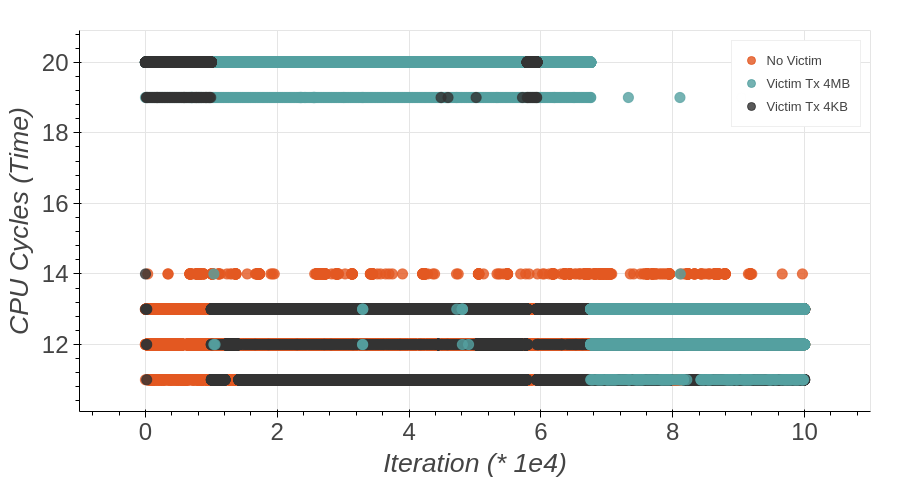
\includegraphics[width=\columnwidth]{figures/interconnect-sc/store-ops/cpu_store_victim_observation.png}
    \caption{Observing the presence of victim DMA traffic using \textit{store} instructions. The victim does $10^4$ iterations of transferring 4KB/4MB.}
    \label{fig:cpu-store-victim-observation}
    % 2025-03-06_14-20
\end{figure}

\subsection{Evaluation}
\label{subsec:interconnect-sc-store-ops-evaluation}

\section{Generating contention via DMA}
\label{sec:interconnect-sc-dma}

In this section, we discuss how an adversary can use direct memory access (DMA) to create contention in the buffers of a PCIe controller.
We revisit \textbf{RQ1} to determine if an adversary can use this approach to observe the victim's traffic pattern. 
In addition, we also provide an answer to \textbf{RQ2} by demonstrating that an adversary can create congestion on a non-hierarchical PCIe 4.0 link.

A DMA controller can generate memory addresses and initiate memory \textit{load} or \textit{store} instructions that are executed in parallel, independent of the execution units of the CPU.
The DMA controller receives commands specifying the source and destination addresses and the size of the data to copy.
Once the data transfer is complete, it issues a notification of completion to the command issuer.
As such, DMA controllers like those on Nvidia GPUs provide a mechanism to measure only the completion time of the entire DMA transfer, not the completion time of individual \textit{load} or \textit{store} instructions.

\subsection{Challenges}
\label{subsec:interconnect-sc-dma-challenges}
\subsection{Using DMA operations to observe presence/absence of victim traffic on PCIe}
\label{subsec:interconnect-sc-dma-evaluation}

Now that we know that the PCIe bandwidth can be saturated with 4MB transfers, we can use this information to craft an adversary that can create congestion in the non-hierarchical PCIe link.
To achieve this, we use the pseudo-code outlined in \Cref{lst:timing-victim-with-dma}.
We assume that the victim is also transferring data to/from the GPU via DMA.

To evaluate our ability to detect victim traffic, we run the adversary for $10^4$ iterations.
At the same time, we execute the victim, which repeatedly (for $10^3$ iterations) performs a DMA transfer of either 4KB or 4MB
As before, we synchronise the execution of the critical code sections responsible for data transfers between the victim and the adversary. 

As shown in \Cref{fig:dma-contention-4mb}, the time it takes to complete the call to \textit{cudaMemcpy} increases in the presence of victim traffic and reduces once the victim stops transmitting.
As such, an adversary is able to determine the presence/absence of victim traffic.

We also explore if the adversary can determine this without saturating the PCIe bandwidth.
For this, we follow the same pseudo-code in \Cref{lst:timing-victim-with-dma}, but set the transfer size of the adversary to 4KB.
As shown in \Cref{fig:dma-contention-4kb}, the adversary can still observe the presence or absence of the victim traffic.

\begin{minipage}{\textwidth}
    \lstinputlisting[language=Python]{code/interconnect-sc/timing-victim-with-dma.py}
    \captionsetup{type=lstlisting}
    \caption{Attacker code to detect presence of victim traffic via DMA operations}
    \label{lst:timing-victim-with-dma}
\end{minipage}

\begin{figure}
     \centering
     
     \begin{subfigure}[b]{\textwidth}
        \centering
        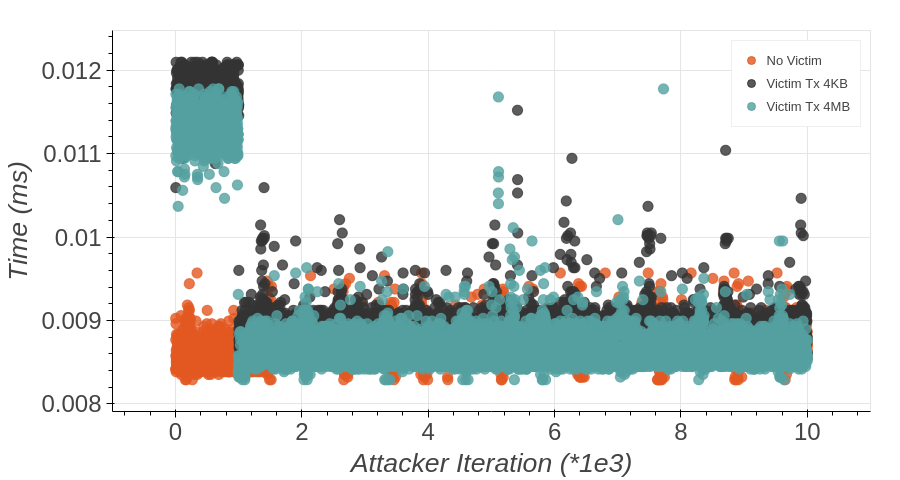
\includegraphics[width=\textwidth]{figures/interconnect-sc/dma/dma_contention_4KB.png}
        \caption{Attacker transfers 4KB}
        \label{fig:dma-contention-4kb}
     \end{subfigure}
     
     \hfill
     
     \begin{subfigure}[b]{\textwidth}
         \centering
        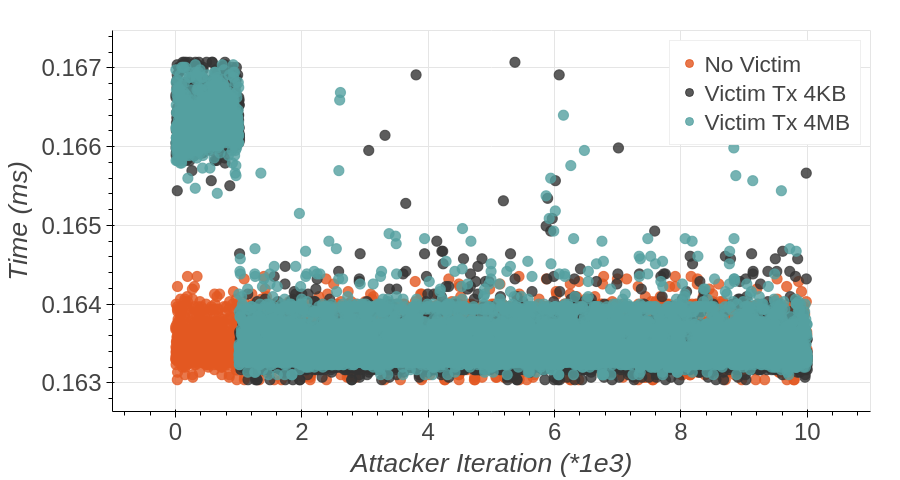
\includegraphics[width=\textwidth]{figures/interconnect-sc/dma/dma_contention_4MB.png}
        \caption{Attacker transfers 4MB}
        \label{fig:dma-contention-4mb}
     \end{subfigure}
     
    \caption{Observing the presence of victim DMA traffic using DMA operations. The victim does $10^3$ iterations of transferring 4KB/4MB.}
    \label{fig:dma-contention}
    % 2025-03-06_17-18
\end{figure}


\section{Limitations}
\label{sec:interconnect-sc-limitations}

Our work has two limitations.
First, in order to carry out a side-channel attack using \textit{store} operations (as outlined in \Cref{sec:interconnect-sc-store-ops}), the attacker requires superuser privileges.
The privileges are required as the attacker needs to map a PCIe resource, which is only available to the root user.
However, it is reasonable to assume that the attacker has these privileges inside their own environment, such as the virtual machine they are running on.
Second, our DMA-based contention mechanism is currently dependent on the round-robin-like scheduling policy that the current DMA controller on the Nvidia A100 GPU currently enforces.
As such, if this policy changes in future GPUs, it is unclear whether the same mechanism would work to observe contention.

In addition, the discussion regarding the behaviour of various hardware components is based on a hypothesis made from the observed behaviour.
It is not possible for us to verify the correctness of our hypothesis as the systems discussed here are proprietary and do not have available public information to verify our conclusions.
\section{Related Work}
\label{sec:interconnect-sc-related-work}

Invisible Probe \cite{tan2021invisible} was the first work to study the security implications of congestion on PCIe.
However, their approach required a hierarchical PCIe topology with a shared PCIe switch or PCH and depended on the attacker saturating the PCIe bandwidth to induce congestion on the PCIe switch or PCH.
\citet{giechaskiel2022cross} follows the same approach as Invisible Probe.
They also attempt to saturate the upstream PCIe bandwidth on a PCIe switch, thus inducing contention on the PCIe switch.
LockedDown \cite{side2022lockeddown} shares the system setup with our work, where the GPU is directly connected to the host.
They also use the DMA controllers on the GPU to transfer data to/from the CPU and create contention.
In contrast, our work shows that the attacker does not need to saturate the PCIe bandwidth to observe contention with the victim's traffic. 
Furthermore, our work establishes that contention can occur even when the combined bandwidth usage of the victim and the attacker remains below saturation.


\begin{singlespace}
\raggedright
\bibliographystyle{abbrvnat}
\bibliography{biblio}
\end{singlespace}

\end{document}
